\documentclass[UTF8]{ctexart}


% \documentclass{article}
\usepackage{amsmath}
\usepackage{listings}
\usepackage{color,xcolor} 
\usepackage{colortbl}
\usepackage{graphicx}
\usepackage{booktabs} %绘制表格
\usepackage{caption2} %标题居中
\usepackage{geometry}
\usepackage{array}
\usepackage{amsmath}
\usepackage{subfigure} 
\usepackage{longtable}
\usepackage{abstract}
\usepackage{multirow}
\usepackage{enumerate}
\usepackage{float}
\usepackage{graphicx}

\usepackage{xltxtra}
\usepackage{mflogo,texnames}
\usepackage{amssymb}
\usepackage[numbers,sort&compress]{natbib}



%伪代码
\usepackage{algorithm}
\usepackage{algpseudocode}
\usepackage{amsmath}
\renewcommand{\algorithmicrequire}{\textbf{输入:}}  % Use Input in the format of Algorithm
\renewcommand{\algorithmicensure}{\textbf{过程:}} % Use Output in the format of Algorithm

\usepackage{xltxtra}
\usepackage{mflogo,texnames}
\usepackage{amssymb}

%附录代码
\usepackage{listings}
\usepackage{xcolor}

\lstset{
    numbers=left, 
    numberstyle= \tiny, 
    keywordstyle= \color{ blue!70},
    commentstyle= \color{red!50!green!50!blue!50}, 
    frame=shadowbox, % 阴影效果
    rulesepcolor= \color{ red!20!green!20!blue!20} ,
    escapeinside=``, % 英文分号中可写入中文
    xleftmargin=2em,xrightmargin=2em, aboveskip=1em,
    framexleftmargin=2em
} 

\pagestyle{plain} %页眉消失

\geometry{a4paper,left=2.5cm,right=2.5cm,top=2.5cm,bottom=2.5cm}%设置页面尺寸
\lstset{
		numbers=left, %设置行号位置
		numberstyle=\tiny, %设置行号大小	
		keywordstyle=\color{blue}, %设置关键字颜色
		commentstyle=\color[cmyk]{1,0,1,0}, %设置注释颜色
		escapeinside=``, %逃逸字符(1左面的键),用于显示中文
		breaklines, %自动折行
		extendedchars=false, %解决代码跨页时,章节标题,页眉等汉字不显示的问题
		xleftmargin=1em,xrightmargin=1em, aboveskip=1em, %设置边距
		tabsize=4, %设置tab空格数
		showspaces=false %不显示空格
	}


		% \begin{figure}[!htbp]\centering
		% \includegraphics[width=1\textwidth]{img} % 图片相对位置
		% \label{fig:figure 0} % 图片标签
		% \end{figure}


\title{\textbf{标题}}
% \date{August 24, 2022}
\date{} %关闭日期时间的显示

\begin{document}
\maketitle{}
\renewcommand{\abstractname}{\Large 摘要\\}   %摘要部分
\begin{abstract}
	\normalsize
    % \CJKfamily{song}
    \fontsize{12pt}{18pt}
	
    玻璃制品是古代中西方文化来往的宝贵物证,具有重要的历史意义。古代玻璃制品易受埋藏环境的影响,内部化学成分的比例发生变化,最终风化。风化与化学成分比例、类型、饰品类别有着密切的关系。本文旨在建立数学模型,以数学的方式对玻璃制品进行成分分析和鉴别。

    针对问题一,对数据进行定性定量分析,利用随机森林算法进行缺失值的填补后用剔除无用的数据,极差化方法去量纲处理。采用卡方检验和斯皮尔曼相关系数分析法进行风化的相关分析,得出风化只跟类型和颜色具有相关性;为探究化学成分的统计规律,在诊断数据有强多重共线性的情况下,建立岭回归分析预测模型,求解出化学成分之间的函数关系式(即统计规律),按照玻璃分类共30条岭回归方程,结果见附录。

    针对问题二,熵值法处理数据得出xxx的分类规律,借鉴生物分类法中的“亚”种群的分类思想建立K-means++和BP神经网络混合模型结合遗传算法寻优,给出亚分类的分类结果,完整数据见附录;根据玻璃类型分两类进行敏感度分析,借助Salib采样多个特征向量预测,分一、二阶和总阶敏感度进行分析。

    针对问题三,对表单三采用随机森林算法填补缺失值,按训练集:测试集为7:3的比例划分数据集,引入集成模型,组合$LGBMClassifier$ 、$LogisticRegression$ 在内的七个模型为基分类器,使用$StackingCV Classif ier$ 进行模型集成,设置五折交叉检验对泛化能力进行评估,穷举寻优找到最优的分类预测结果,对表单三中未分类的样品进行了预测,结果见附录。

    针对问题四,


	\textbf{关键字}: ;  ;  ;  ;  ;   %关键词
\end{abstract}
\thispagestyle{empty}    %该页不编码且独立为一页
\newpage

\setcounter{page}{1}  %此页开始编码

%第一部分
\section{问题重述}

\subsection{问题背景}
路上丝绸之路起源于西汉时期,是古代中西方文化交流的通道,其中的玻璃制品是早期贸易往来的宝贵物证,凝结着古代劳动人民的智慧和艺术以及高超的工艺技术,体现着中西方文化交互的往来。
有些历史悠久的宝贵玻璃制品可视为中华文化的瑰宝,便有了许多考古工作者对其进行成品分析与鉴别。改革开放以来新中国对珍贵的文物提出了许多保护的法案,如1982年《文物保护法》,就将玻璃制品在内的文物保护以法律形式固定。

玻璃的主要原料是石英砂,在炼制的过程中加入了助熔剂,由于其助熔剂成分的不同导致其主要化学成分不同。
本文主要涉及铅钡玻璃和钾玻璃,其中铅钡玻璃通常被认为是我国自己发明的。古代的玻璃制品在埋藏以及其埋藏的环境等多种因素的影响下
而导致风化,即玻璃内部与环境之间产生大量的元素交换,使其内部的成分比例发生变化。风化的玻璃制品根据分析表面的化学元素
以及颜色等佐助依据判断出风化区域以及
可能存在的未风化区域。考古学者根据对不同类型以及风化与否的玻璃制品进行采样得出其化学成分占比,
其和理应为100$\%$,由于存在误差,给定有效范围为85$\%$$ \sim $ 105$\%$。


\subsection{问题提出}
根据以上的背景,以及给出的附录,建立模型解决以下问题:

1.研究玻璃文物表面风化和类型、纹饰、颜色的关系;结合其类型分析表面风化情况和化学成分含量之间的统计规律;并根据风化点的数据预测未风化时的化学成分含量。

2.分析高钾和铅钡玻璃的分类规律;对不同类别选择合适的化学成分进行亚分类,并分析其合理性和敏感性。

3.对附录中的表单三进行玻璃类型鉴别,并分析其结果的敏感性。

4.对不同类别的样品,分析化学成分之间的关系,并比较不同类别间的有何差异性。

% \hspace*{\fill}

其中,附录表单一给出的为玻璃文物的基本信息;表单二为对已分类玻璃文物采样的化学成分比例,同一样品的不同部位的检测值可能存在差异;
表单三为未分类玻璃文物的化学成分比例。



%第二部分
\section{问题分析}
\subsection{问题一的分析}
问题一首先要求根据附录表单一的数据研究玻璃文物的表面风化和类型、纹饰、颜色的关系,探究其关系则需进行定量分析,以数学的语言来进行描述。其次要求结合类型来分析表面风化情况和其化学成分含量之间的统计规律,最后能够根据风化点的数据预测其未风化前的化学成分含量。在统计领域中,统计规律指的是对大量偶然事件整体起作用的规律,表现这些事物整体的本质和必然的联系。
在此我们理解为数学表达式,即关系方程。

首先对数据进行观测和筛选处理,对于研究风化和类型、纹饰、颜色之间的关系,需对其进行卡方检验,并观察其结果。考虑到其数据值为定类,不服从正态分布故采取斯皮尔曼相关系数法进行分析,来得出其相关性的结论。其次分析数据的线性关系,通过共线性诊断后,决定采用岭回归分析来构建回归方程用以描述表面风化情况和其化学成分含量之间的统计规律。最后在已有回归方程的基础上通过控制变量法进行预测未风化时的化学成分含量。



\subsection{问题二的分析}
问题二首先要求我们依据附录分析出高钾和铅钡两种玻璃的分类规律;其次要根据不同的类别的玻璃制品分析选择合适的化学成分进行分析,并对其进行亚类划分;
最后对分类的结果进行检验,分析合理性和模型的敏感性。 该问主要问题在于亚类划分,亚类在专业术语中属于土类的一种划分类别名词,较难解释关系。
在此问之中我们引入对生物类别划分中的“亚”种分类,对玻璃制品风化情况进行亚类划分。

首先考虑有的成分对整体结果的影响可能不大,为了降维而采用$PCA$(主成分分析法)进行数据处理,但在发现进行数据拟合的时候
其准确率不如未处理前,故基础数据不予以降维处理。其次,对比$K-means++$聚类、层次聚类、随机森林分类几种方法后,决定采取效果较好的$K-means++$聚类—$BP$神经网络混合模型对不同类别的
玻璃制品进行划分分类。





\subsection{问题三的分析}
问题三要求针对附录表单三中未知玻璃类型的文物样品数据进行化学成分之间的分析,通过分析来确定其玻璃类型,
最后需对鉴别的结果进行敏感性分析。 该问也是预测问题,根据给出的数据进行分析后进行预测其玻璃类型。

首先,仍采用在第一问中使用过的随机森林算法进行填补,后对数据的定类转化为定量。采用集成学习模型来进行预测鉴别,它通过组合多个模型来进行预测,在集成成员构建正确的情况下,有效的提高最终集成的性能,能够更好的解决不同应用中的不均衡数据集问题。我们构建基于$LGBMClassifier$, $LogisticRegression$, $AdaBoostClassifier$, $StackingClassifier$等七个模型所搭建的集成学习模型。经过$Exhaustive search$对模型进行超参寻优,使用五折交叉验证进行泛化能力的评估。最后使用全部的数据集进行训练,最终再对玻璃样品进行类型预测。


\subsection{问题四的分析}
问题四要求针对不同的类别的玻璃文物样品,分析其化学成分之间的关联关系,通过对成分之间的关联关系的
发掘确定其关联的具体情况,最后需要对各个不同类别的化学成分的关联关系的差异性进行分析。该问是一种关联性及擦会议下分析
问题,根据提供的数据对成分之间的关系进行构建分析。

首先对数据进行类别分析。因为在提供的数据中只有类型、纹饰、颜色、
表面风化、采样点和成分六个属性。而在第一问中,已经通过模型检验
出类型和表面风化有着较强的相关性和显著性差异。因此类别首先细分为
高钾、铅钡两种类型,其次依据是否表面风化决定归于哪一个类别。
接着对数据进行归一化操作后,判断数据是否服从正太分布和是否线性;
判断完成后进行灰色关联分析得到成分之间的关联关系;随后进行
多配对样本Friedman检验-Nemenyi后续检验,分析出成分之间的关联关系的差异性

%第三部分
\section{模型假设}
1.假设......................

2.

3.

4.

5.

6.

%第四部分
\section{符号说明}


		\begin{table}[H] 
		\begin{center}  
		\begin{tabular}{c|c|c}    
		\toprule[2pt]    
		\rowcolor[gray]{0.8}

		\multicolumn{1}{m{8em}}{\centering 符号}  &\multicolumn{1}{m{15em}}{\centering 基本说明} &\multicolumn{1}{m{10em}}{\centering 单位}\\

		%直接用合并单元格的方法来实现自定义列宽的同时,使文字居中对齐

		\midrule[1.3pt]
		    $\alpha$                                & x        & | \\
			$\lambda$                                & x        & |       \\
			$\theta$                                 & x        & |            \\


		\bottomrule[2pt]   
		\end{tabular}  
		\end{center}
		\end{table}




%第五部分
\section{问题一的模型建立与求解}
\subsection{问题分析}
本问可细分为三小问,1.研究玻璃文物表面风化和类型、纹饰、颜色的关系;2.探究类型以及风化情况和化学成分之间的统计规律;
3.预测已风化样品未风化前的化学成分含量。

第一,考虑到数据给出有范围,需要进行数据筛选以及对缺失值的处理(此处采用随机森林进行填充),根据其数据为定类的特征
进行卡方检验分析其显著性;采用斯皮尔曼相关系数法分析相关性。

第二,求解类型以及风化情况与化学成分之间的统计规律,对统计学中统计规律这一概念的理解,我们解释为获取一个相关的函数方程,
用以解释类型以及风化情况和化学成分之间所存在的统计规律。数据指标之间可能存在共线性关系,因此采用岭回归分析,得到其函数方程。

第三,在已经搭建好的岭回归模型的基础上,通过改变变量的值来达到对已风化的样品进行风化前的化学成分预测。

具体思路的流程图如下:
\begin{figure}[H]\centering
	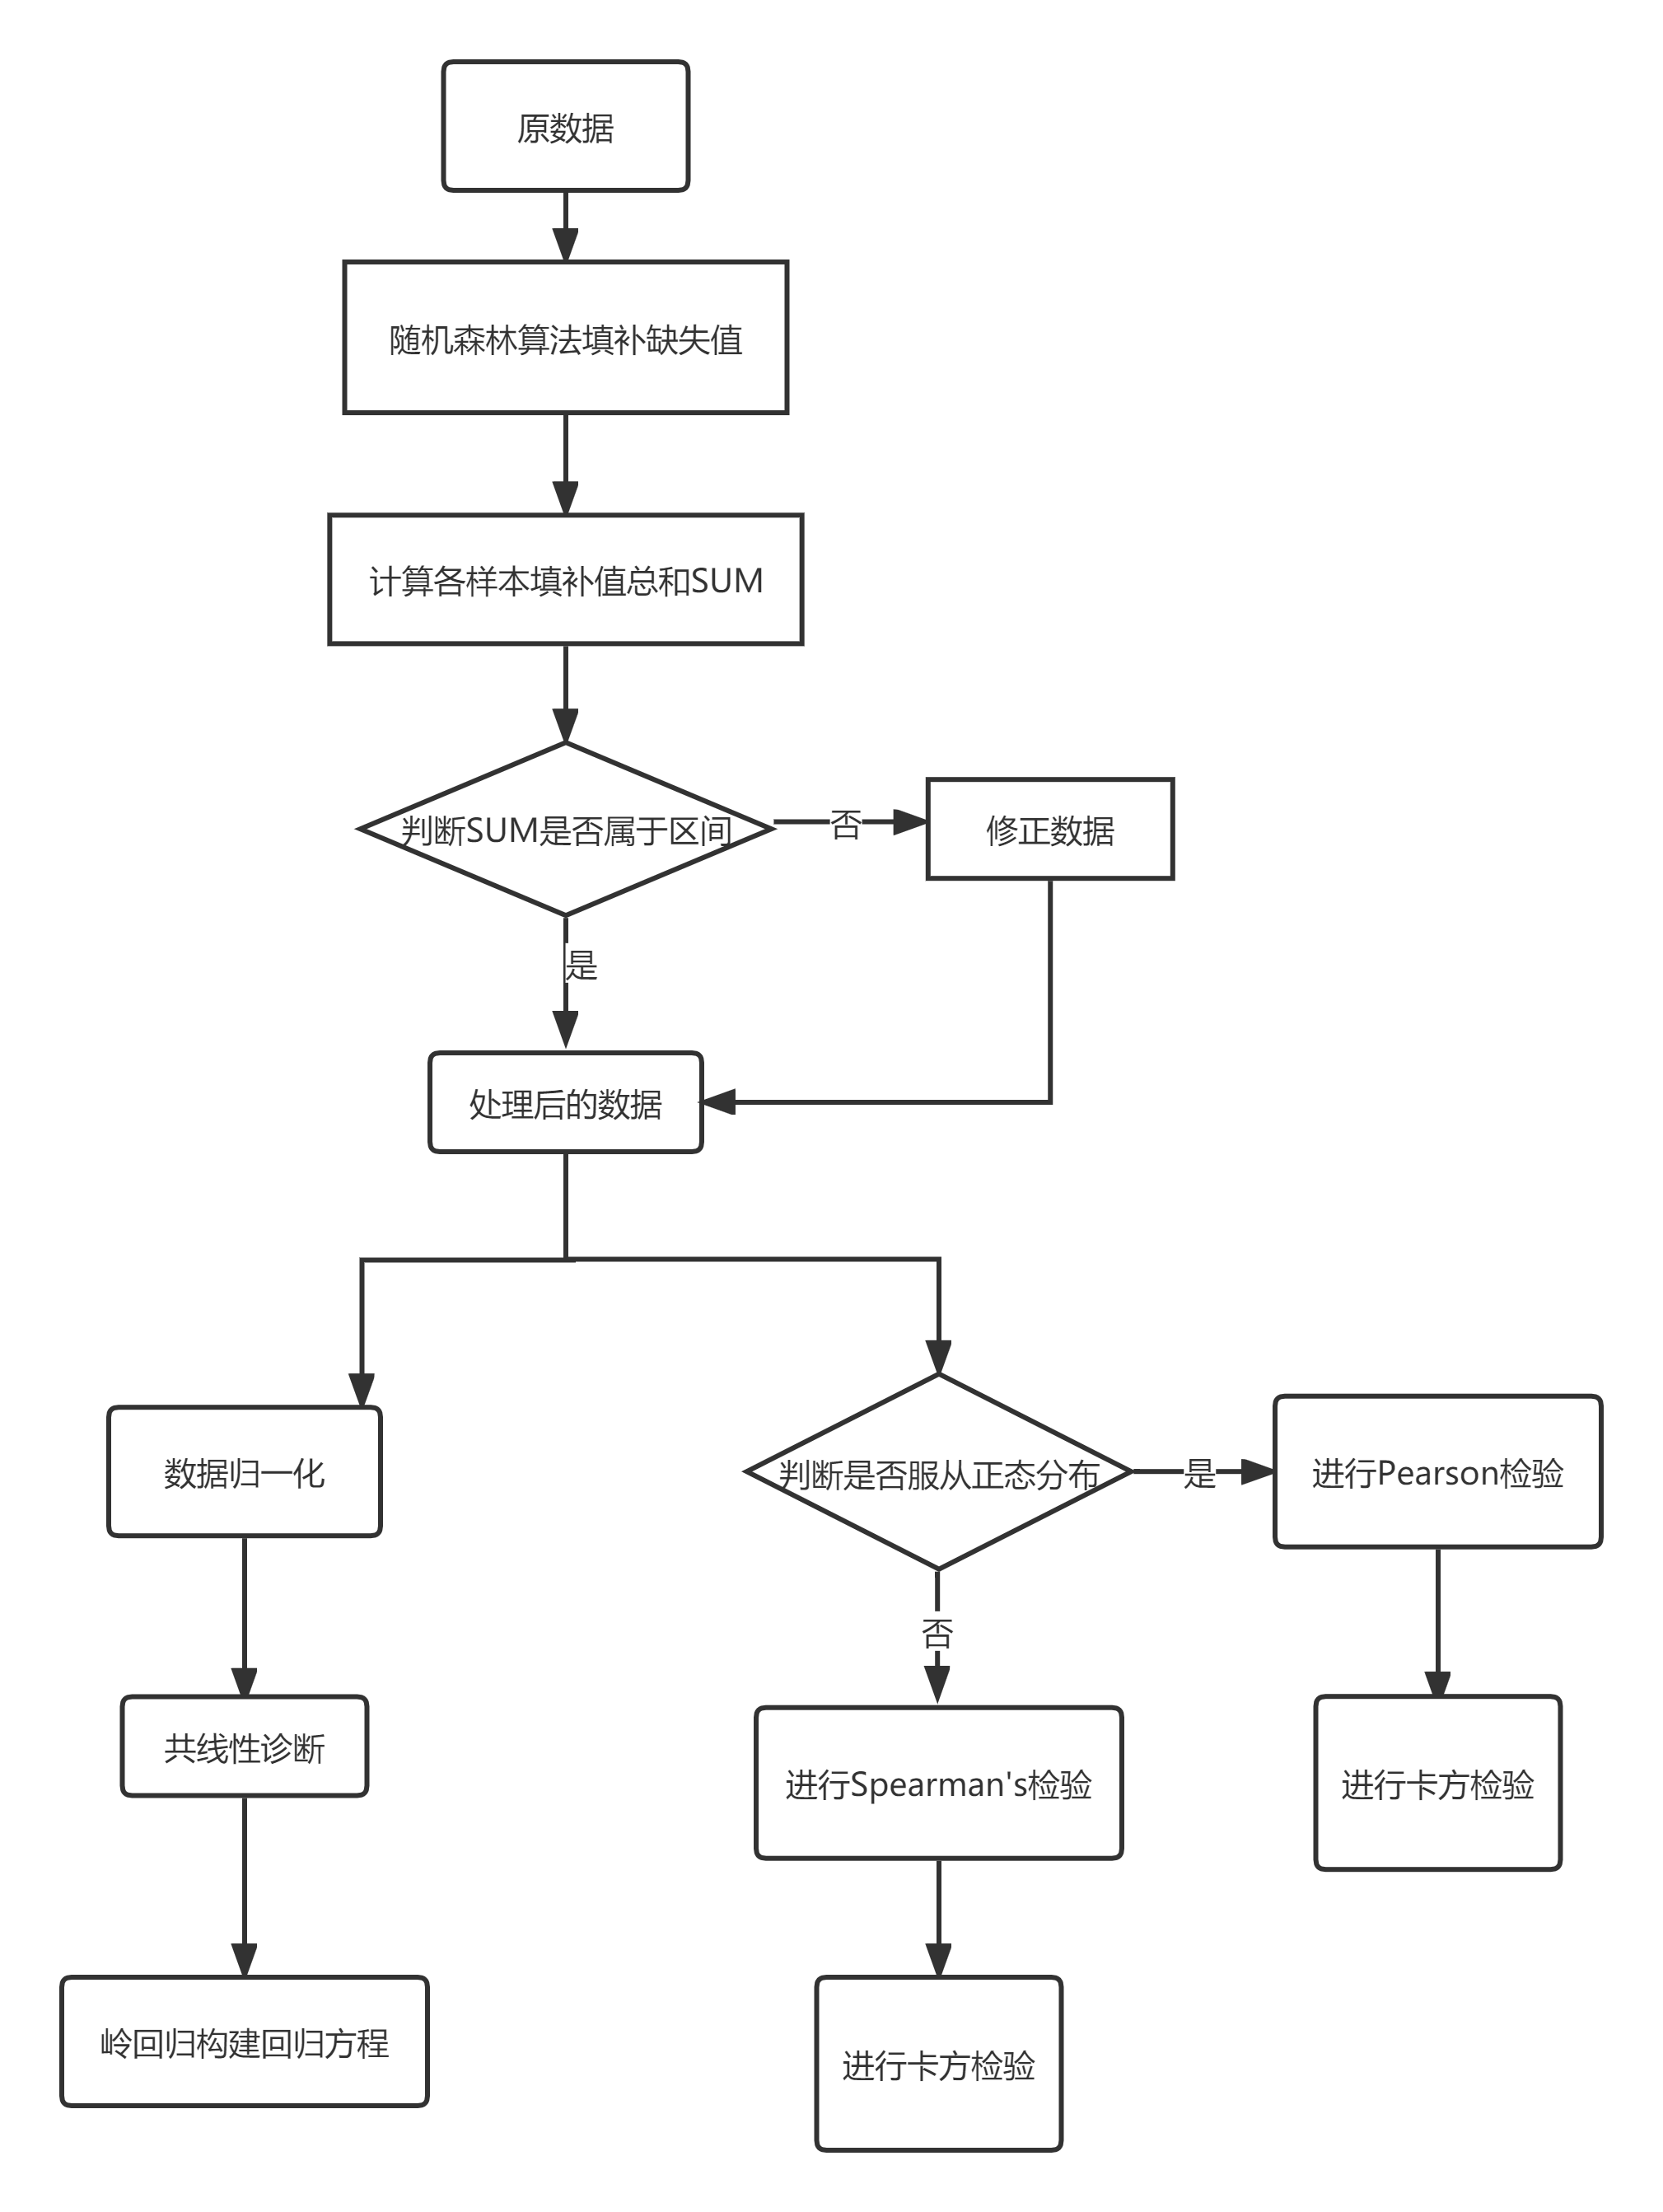
\includegraphics[width=0.5\textwidth,height=0.55\textwidth]{img/第一问流程图.png} % 图片相对位置 
	\caption{求解类型和风化情况与化学成分之间的统计规律} % 图片标题 
	\label{fig:figure 1} % 图片标签
\end{figure}


\subsection{数据处理}
\subsubsection{剔除无效值}
题目给出了化学成分比例总和的一定范围为:85$\%$$ \sim $ 105$\%$,通过Excel软件对附录中表单一的数据进行求和,处理掉不合规格的数据。

其次,根据题目给出的信息,铅钡玻璃的铅钡含量以及高钾玻璃的钾含量都是相对较高的。考虑到风化的情况会影响它们的成分比例,
可能存在化学反应使其风化后失去了原本含量较高的铅钡或者钾元素,据此可得出结论:其不同类型的玻璃样品在其风化前,对应类型
的化学成分(铅钡或钾)应该有一定的占比。根据结论可以筛选掉不同类型的玻璃制品其风化前的对应化学成分为零的数据。



\subsubsection{数据归一化处理}
由于相同的数据指标之间可能存在不同的量纲和量纲单位,从而影响整体的数据分析和建模后的求解。为了让数据指标在同一数量级
和消除量纲,使得数据之间可比,采用了归一化处理,本文用的是最大-最小标准化。在数量为$n$数据集$A$中排序选出最大值$maxA$和最小值$minA$,
则集合中的元素$a_i$通过最大-最小标准化可以映射为:
\begin{equation}
	a_i = \frac{a_i-minA}{maxA-minA}
\end{equation}


通过公式即可对给出的数据进行处理。
\subsubsection{随机森林补全缺失值}
\textbf{Step1: 算法介绍}

给出附录的数据中有着许多空白值,题目给出的解释为检测不到该成分。考虑到由于考古工作者的人工误差,导致检测不到这些数据,
我们采用随机森林算法对这些数据集进行缺失值的填补。随机森林是通过集成学习的$Bagging$思想将多棵树集成的一种算法,
其填补过程有两个特点:1.优先填补缺失值较多的;2.通过许多决策树构成森林,依据机器学习进行投票最后确定预测的结果。
如下为决策森林结构图:
\begin{figure}[H]\centering
	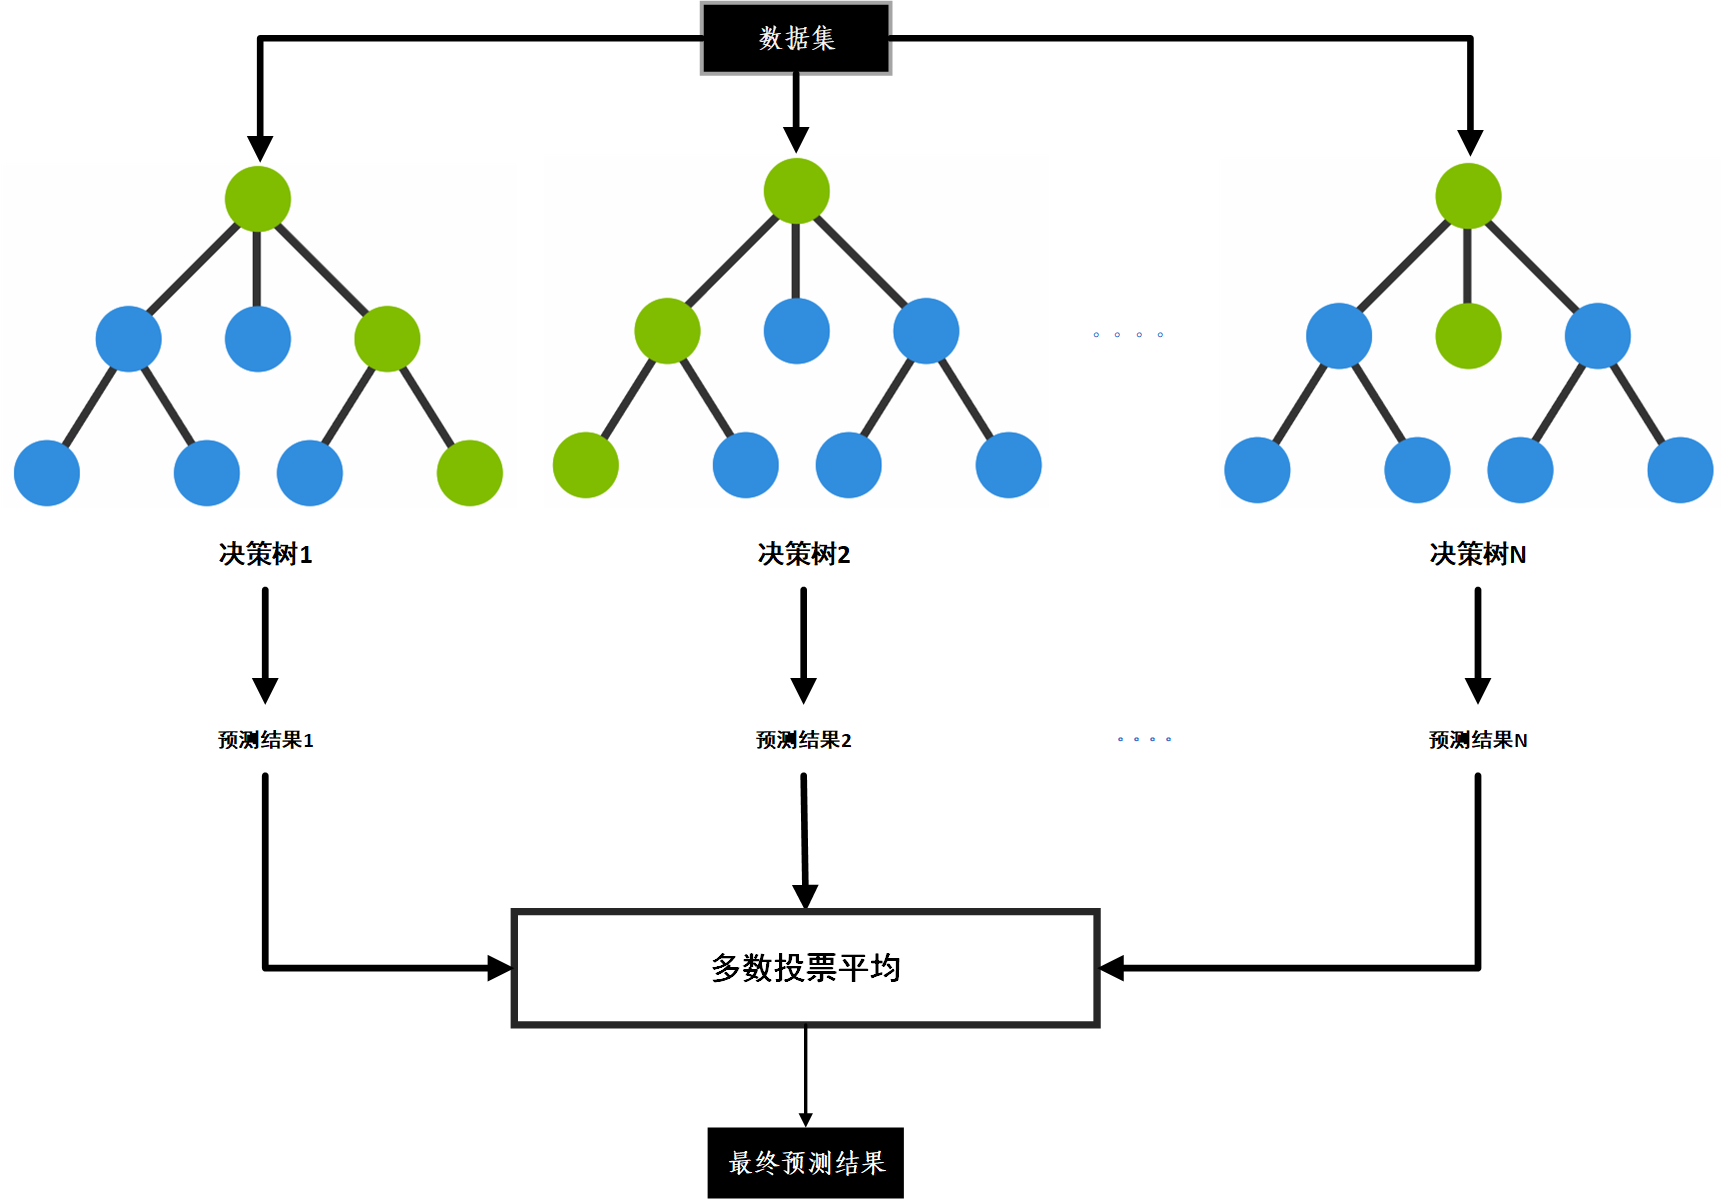
\includegraphics[width=1\textwidth]{img/rf.png} % 图片相对位置 
	\caption{决策森林} % 图片标题 
	\label{fig:figure 1} % 图片标签
\end{figure}


% 通过热量图的分析,得出缺失值的分布情况:

% \begin{figure}[H]\centering
% 	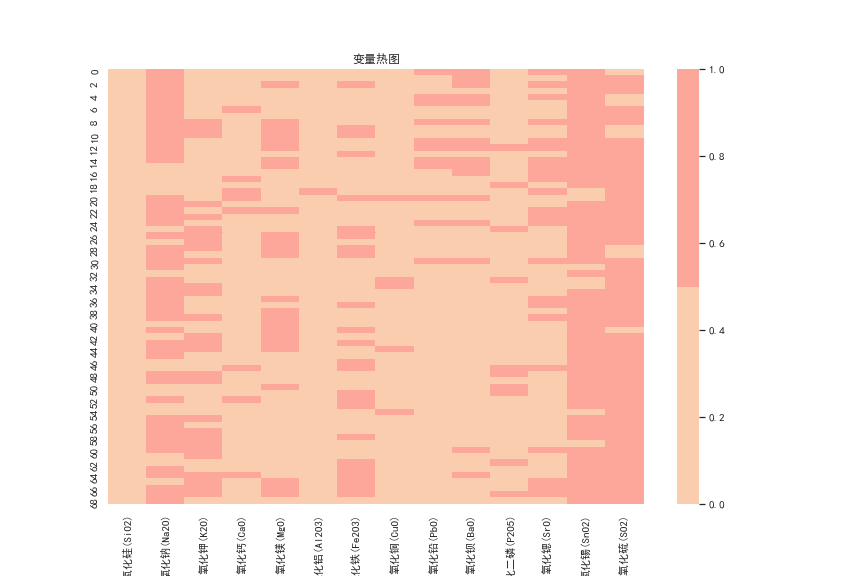
\includegraphics[width=0.6\textwidth]{img/缺失值热力分布.tmp} % 图片相对位置 
% 	\caption{缺失值热力分布} % 图片标题 
% 	\label{fig:figure 2} % 图片标签
% \end{figure}

\textbf{Step2: 数据填补}

通过决策森林的投票决策机制来对缺失值的填补,得出新的结果。求和后发现其比例之和会有一些值超出$105 \% $的范围,对此需要
做进一步的数据处理。首先对原数据进行统计,得出结果:

\begin{figure}[H]\centering
	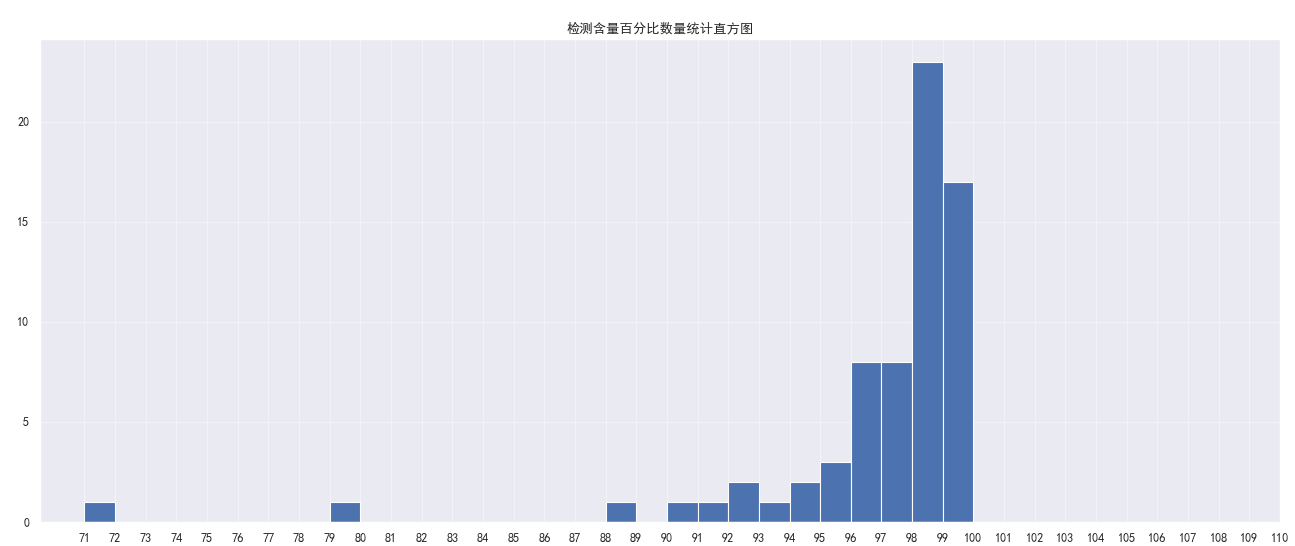
\includegraphics[width=1\textwidth,height=0.48\textwidth]{img/成分比例求和直方图.png} % 图片相对位置 
	\caption{成分比例求和直方图} % 图片标题 
	\label{fig:figure 2} % 图片标签
\end{figure}

通过分析得出大多数的成分比例和都落在98 $\sim$ 100左右,结合范围85$\%$ $\sim $ 105$\%$,我们决定以100作为一个靶值来进行误差的处理。
经查阅文献\cite{ref1} 可知,由于人工以及机器的原因会导致在文物成分采样时存在一定的偏差,可经过算法来进行修正,结合文献所提误差范围来看我们将
误差范围控制在0$\%$ $\sim$ 2 $\%$之间。设补全后的成分求和比例为$Sum$,给出如下的误差$diff$方程:
	\[\left\{\begin{array}{llcl}
		diff = 100-Sum,  \qquad (Sum \le 100) \\
		diff = 2, \qquad \qquad \qquad  \  (Sum>100)
		% S(t_0)&=&140005\times10^4&\text{人},\\
		% I(t_0)&=&14052 &\text{人},\\
		% R(t_0)&=&130 &\text{人},\\
		% Y(t_0)&=&4562 &\text{人},\\
		% N(t_0)&=&6336 &\text{人},\\
		\end{array} \right.\]

根据预测填补后的成分比例对$diff$进行重新的按分配,这就是填补值所产生的可接受误差,最终得出缺失值填补后的数据,数据详见附录。


\subsection{数据分析}
\subsubsection{卡方检验观测显著性}
分析得出数据是不依赖于总体的分布或参数,则非参数检验,所给出的数据为离散型数据(即定类),故采用卡方检验来观测其显著程度。

根据卡方分布定义,若k个随机变量$Z_1$\dots $Z_k$是相互独立,符合标准正态分布的随机变量(数学期望为0、方差为1),则随机变量$Z$的平方和$X=\sum_{i=1}^k$,
被称为服从自由度为$K$的卡方分布,记作$X \sim \chi ^2(k)$。其统计量公式为:
\begin{equation}
	X=\sum_{i=1}^n \frac{(f_i-t_i)^2}{t_i} 	
\end{equation}

其中的$f_i$为观察值,$t_i$为期望值。

通过卡方检验是否呈现显著性($p$值小于0.05或0.01,严格为0.01,不严格为0.05)。其得出的检验结果如下:

\begin{table}[H]
    \centering
	\caption{卡方分析}%图表标题
    \begin{tabular}{|c|c|c|c|c|c|c|c|} \hline
	\multirow{2}{*}{题目} & \multirow{2}{*}{名称} & \multicolumn{2}{|c|}{表面风化} & \multirow{2}{*}{总计} & \multirow{2}{*}{X²} & \multirow{2}{*}{校正X²} & \multirow{2}{*}{P} \\ \cline{3-4}
	&  & 无风化 & 风化 &  &  &  &  \\ \hline
	\multirow{3}{*}{纹饰} & 1 & 13 & 17 & 30 & \multirow{3}{*}{4.957} & \multirow{3}{*}{4.957} & \multirow{3}{*}{0.084*} \\ \cline{2-5}
         & 2 & 11 & 11 & 22 & ~ & ~ & ~ \\ \cline{2-5}
         & 3 & 0 & 6 & 6 & ~ & ~ & ~ \\ \hline
	\multirow{2}{*}{类型} & 1 & 12 & 6 & 18 & \multirow{2}{*}{6.88} & \multirow{2}{*}{5.452} & \multirow{2}{*}{0.009***} \\ \cline{2-5} 
        ~ & 2 & 12 & 28 & 40 & ~ & ~ & ~ \\ \hline
    \multirow{8}{*}{类型} & 1 & 6 & 9 & 15 & \multirow{8}{*}{7.234} & \multirow{8}{*}{7.234} & \multirow{8}{*}{0.405} \\ \cline{2-5}
        ~ & 2 & 8 & 16 & 24 & ~ & ~ & ~ \\ \cline{2-5}
        ~ & 3 & 2 & 2 & 4 & ~ & ~ & ~ \\ \cline{2-5}
        ~ & 4 & 3 & 4 & 7 & ~ & ~ & ~ \\\cline{2-5}
        ~ & 5 & 2 & 0 & 2 & ~ & ~ & ~ \\ \cline{2-5}
        ~ & 7 & 2 & 1 & 3 & ~ & ~ & ~ \\ \cline{2-5}
        ~ & 8 & 0 & 2 & 2 & ~ & ~ & ~ \\ \cline{2-5}
        ~ & 9 & 1 & 0 & 1 & ~ & ~ & ~ \\ \hline
    \end{tabular}
\end{table}

	

根据上述得出的结论为:

(1)$P$值为0.084*,表面风化和纹饰数据不存在显著性差异

(2)显著性$P$值为0.009***,表面风化和类型数据存在显著性差异

(3)显著性$P$值为0.405,表面风化和颜色数据不存在显著性差异

表注:***、**、*分别代表1$\%$、5$\%$、10$\%$的显著性水平
\subsubsection{斯皮尔曼相关系数分析}
查阅资料发现皮尔森相关系数和斯皮尔曼相关系数可以描述两组变量相关性\cite{ref2} 。两者相比斯皮尔曼
相关系数不需要数据服从正态分布,所以在分析理论中,斯皮尔曼相关系数的应用相对广泛,
用以衡量变量之间的依赖性的非参数指标。分析表面风化和类型、纹饰、颜色这些数据得出明显是离散型变量,采用斯皮尔曼相关分析是合理的。
下面给出构建过程:

设$X$、$Y$为两组独立同分布的数据,其元素个数均为$N$,两组随机变量中取的第$i$个值分别用$X_i$、$Y_i$表示。对序列进行排序,
得到集合$x$和$y$,相同$i$的$x$和$y$元素的差值排行差分集合为$d$。则相关系数$r_s$可表示为:
\begin{equation}
	r_s=\frac{\sum_{i=1}^N(x_i-\overline{x})(y_i-\overline{y})}{\sqrt{\sum_{i=1}^N(x_i-\overline{x})^2 \sum_{i=1}^N(y_i-\overline{y})^2} }
\end{equation}

相关系数$r_s$取值范围在[-1,1],其正负也代表着正负相关性。若总体的相关系数$\varrho =0$,则相关系数$r_s$分布可近似的用均值表示
为0,标准差为$\frac{1}{\sqrt{n-1} }$正态分布曲线来表示$此处加入引用$,经过变化得到标准正态分布曲线,正态检验值如下:
\begin{equation}
	r_s \sqrt{n-1} \sim N(0,1)
\end{equation}

\begin{equation}
	z=r_s \sqrt{n-1}
\end{equation}

本文所得$P$值合理,故作为斯皮尔曼检验的结果,热力相关图如下:
\begin{figure}[H]\centering
	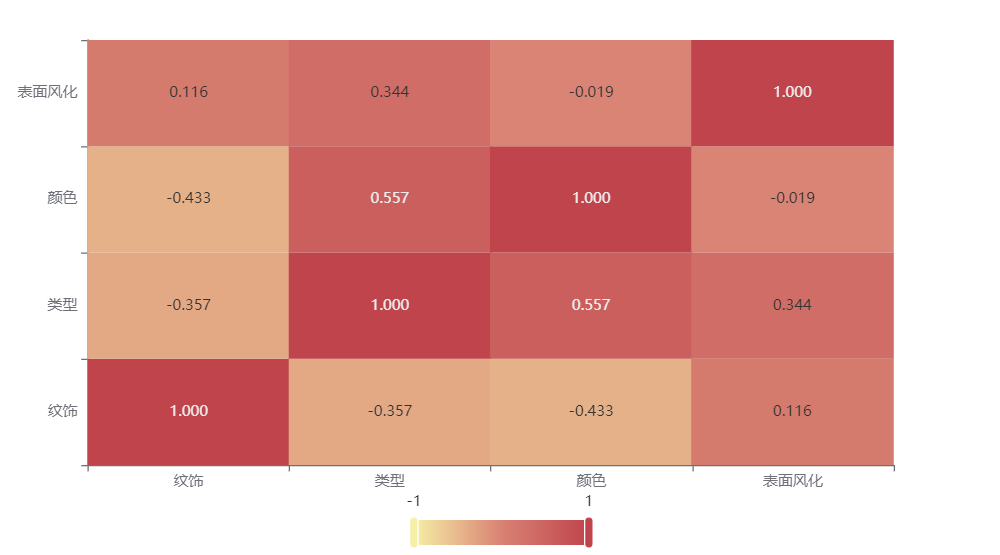
\includegraphics[width=0.8\textwidth]{img/斯皮尔曼相关系数热力图.png} % 图片相对位置 
	\caption{斯皮尔曼相关系数热力图} % 图片标题 
	\label{fig:figure 3} % 图片标签
\end{figure}

根据上述得出的结论为:表面风化与纹饰、类型存在正相关,和颜色为负相关。

\subsection{岭回归分析预测模型的建立}
\subsubsection{模型确立}
岭回归模型适用解决多重共线性的有偏估计回归方法,其本质是一种改良的最小二乘估计,通过放弃最小二乘的无偏性, 
以损失部分信息和降低精度为代价获得回归系数更符合实际、可靠的回归方法。其约束自变量来解决数据集之间具有的多重共线性的问题,
即预测变量之间具有相关性的问题。与一般的最小二乘估计以及线性回归方程有着补加项的区别,能够改良损失函数,得到更好的结果。

\subsubsection{多重共线性诊断}
根据上述的分析可知,岭回归模型适用于多重共线性的有偏估计,为证明采用该模型的合理性,需要对化学成分数据进行多重共线性诊断,
来判断模型选取是否合理。

多重共线性定位为:线性回归模型中变量之间因为存在精确或高度的相关关系使得模型估计和拟合不合理,得不到理想的结果,简言之
多重共线性就是自变量之间存在着线性相关性,导致在回归中得不到理想的结果。利用SPSS软件对包括风化情况在内的15个指标进行共线性
诊断采取依次压入法,即一次输入一个成分,分析剩余成分与其之间的关系如何。

注:此文对风化情况进行数学化处理,风化为1,无风化是0。

由于结果过多,此处仅展示二氧化硅此化学成分和其余自变量的多重共线性,其余数据在附录中。
\begin{table}[H]
    \centering
	\caption{多重共线性诊断的VIF图}
    \begin{tabular}{|c|c|c|c|c|c|c|c|} \hline
	\multirow{2}{*}{模型} & \multicolumn{2}{|c|}{非标准化系数} & \multicolumn{2}{|c|}{共线性统计} & \multirow{2}{*}{标准化系数Beta} & \multirow{2}{*}{t} & \multirow{2}{*}{显著性} \\ \cline{2-5}
	~ & B & 标准错误 & 容差 & VIF &  &  &  \\ \hline
	常量 & 0.072 & 0.007 & ~ & ~ & ~ & 10.206 & 0.009 \\ \hline
    $x_{2}$ & -0.020 & 0.020 & 0.003 & 354.187 & -0.136 & -0.995 & 0.425 \\ \hline
    $x_{3}$ & -0.063 & 0.050 & 0.001 & 745.339 & -0.247 & -1.246 & 0.339 \\ \hline
	$x_{4}$ & -0.045 & 0.033 & 0.002 & 404.665 & -0.204 & -1.394 & 0.298 \\ \hline
    $x_{5}$ & -0.026 & 0.021 & 0.005 & 187.212 & -0.124 & -1.250 & 0.338 \\ \hline
    $x_{6}$ & -0.049 & 0.063 & 0.001 & 785.799 & -0.161 & -0.789 & 0.513 \\ \hline
    $x_{7}$ & -0.020 & 0.022 & 0.003 & 344.463 & -0.121 & -0.896 & 0.465 \\ \hline
    $x_{8}$ & -0.032 & 0.007 & 0.092 & 10.927 & -0.120 & -4.982 & 0.038 \\ \hline
    $x_{9}$ & -0.002 & 0.006 & 0.042 & 23.930 & -0.010 & -0.284 & 0.803 \\ \hline
    $x_{10}$ & -0.004 & 0.011 & 0.009 & 114.343 & -0.024 & -0.313 & 0.784 \\ \hline
    $x_{11}$ & -0.003 & 0.012 & 0.009 & 106.185 & -0.019 & -0.253 & 0.824 \\ \hline
	$x_{12}$ & -0.006 & 0.029 & 0.002 & 604.627 & -0.039 & -0.216 & 0.849 \\ \hline
	$x_{13}$ & -0.002 & 0.007 & 0.007 & 141.708 & -0.026 & -0.295 & 0.795 \\ \hline
	$x_{14}$ & -0.003 & 0.011 & 0.010 & 98.765 & -0.019 & -0.262 & 0.818 \\ \hline
	$x_{15}$ & 0.002 & 0.03 & 0.003 & 297.972 & 0.097 & 0.769 & 0.522 \\ \hline
    \end{tabular}
\end{table}

通过VIF的大小来判断多重共线性的强弱, 通常以10作为边界, 1.当$VIF<10$,不存在多重共线性;$10<=VIF<100$, 存在较强的多重共线性; $VIF>=100$, 则存在严重多重共线性.
通过上图分析,基本全部数据都呈现了很强的多重共线性问题,其余化学成分的检测结果也都呈现了自变量之间存在着很强的多重共线性。
故在模型选择上,选择岭回归模型是合理的。

\subsubsection{模型构建}
一般线性回归方程表示为$Y=\sum_{i=1}^p \beta_i X_i + \beta_0$ ($p$为样本点总数,$\beta_i$为待求系数,$\beta_0$为偏差)。
普通的最小二乘法最小化偏差公式为:
\begin{equation}
	\hat{\beta } = \min \sum_{i=1}^p(Y_i-\beta_0 - \sum_{i=1}^p \beta_i X_i)^2
\end{equation}

为了消除数据间的共线性添加一项惩罚项$\lambda \sum_{i=1}^p \beta_{j}^2$从而得到岭回归公式如下:
\begin{equation}
	\hat{\beta } = [\min \sum_{i=1}^p(Y_i-\beta_0 - \sum_{i=1}^p \beta_i X_i)^2 + \lambda \sum_{i=1}^p \beta_{j}^2]
\end{equation}

该函数性质上为一个凸函数,其中当$\frac{\partial \widehat{\beta} }{\partial \beta}=0$时,函数取得最小值:
\begin{equation}
	\beta_{min} = (X^T X+\lambda I)^{-1} X^T Y
\end{equation}

其中$\hat{\beta }$为偏差值,$\lambda$为岭系数,$\beta_{j}$为损失函数,$X^T$为$X$的转置,$I$为单位矩阵。根据上述得出的结论为
(3)式即可进行分析求解。




\subsection{岭回归分析预测模型的求解}
\subsubsection{模型求解分析}
通过共线性诊断后明确岭回归分析预测模型的选择合理性,该模型是在最小二乘回归的基础上加上了项惩罚项$\lambda \sum_{i=1}^p \beta_{j}^2$,
保证了$\beta$值不会很大,将无偏估计转为有偏估计,有效的解决了多重共线性带来的方程拟合不理想的问题。

本问运用岭回归分析预测模型解决的主要问题是类型以及风化情况和化学成分之间所存在的统计规律,以方程的形式反映数据指标之间的统计规律。
细分后根据玻璃类型和风化情况以及14项
化学指标,可以得出30种分类,需要依次取出一个化学指标作为因变量,剩下的指标作为自变量(含风化情况),
做岭回归分析。由于数量过多,此处仅展示二氧化硅此化学成分的求解过程,其余化学成分的求解结果则在附录中
呈现。

约定二氧化硅、氧化钠、氧化钾、氧化钙、氧化镁、氧化铝、氧化铁、氧化铜、氧化铁、
氧化铅、氧化钡、五氧化二磷、氧化锶、氧化锡、二氧化硫、表面风化这些数据指标以$x_1$,$x_2$,$x_3$ \dots $x_{16}$表示。
其对应的岭回归方程以$Y_1$,$Y_2$,$Y_3$ \dots $Y_{15}$表示。

\subsubsection{求解过程}
\textbf{Step1: 结合岭迹图确定$K$值}

$K$的确定是依据各个自变量的标准化回归系数趋于稳定时的最小$K$值。一般情况下,其值越小偏差也越小。通过
SPSSPro软件得到二氧化硅的岭迹图如下:
\begin{figure}[H]\centering
	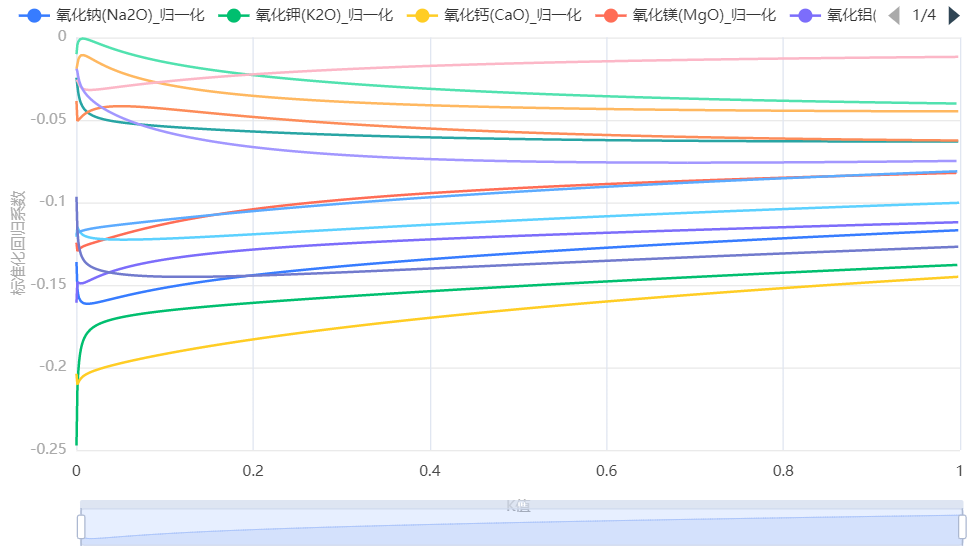
\includegraphics[width=0.9\textwidth]{img/二氧化硅岭迹图.png} % 图片相对位置 
	\caption{二氧化硅岭迹图} % 图片标题 
	\label{fig:figure 5} % 图片标签
\end{figure}

通过上图分析得各个自变量的标准化系数基本趋于稳定。根据方差扩大因子法确定$K=0.129$。	

\textbf{Step2:分析$F$和$R^2$}

分析模型的是否有意义,可以通过分析$F$值来确定,观察$p<0.01$或者$0.5$来判断显著性从而确定是否存在回归关系。 	
如下表所示:
\begin{table}[H]
    \centering
	\caption{岭回归分析输出结果}
    \begin{tabular}{|c|c|c|c|c|c|c|c|c|}
    \hline
	\multirow{2}{*}{K=0.129} & \multicolumn{2}{|c|}{非标准化系数} & \multirow{2}{*}{标准化系数Beta} & \multirow{2}{*}{t} & \multirow{2}{*}{p} & \multirow{2}{*}{$R^{2}$} & \multirow{2}{*}{\text{调整}$R^{2}$} & \multirow{2}{*}{F} \\ \cline{2-3}
        ~ & B & 标准误 & ~ & ~ & ~ & ~ & ~ & ~ \\ \hline
        常量 & 0.079 & 0.001 & - & 86.744 & 0.000*** & \multirow{15}{*}{0.999} & \multirow{15}{*}{0.99} & \multirow{15}{*}{112.891(0.009***)} \\ \cline{1-6}
		$x_{2}$ & -0.022 & 0.004 & -0.149 & -5.904 & 0.028** & ~ & ~ & ~ \\ \cline{1-6}
        $x_{3}$ & -0.042 & 0.004 & -0.164 & -10.158 & 0.010*** & ~ & ~ & ~ \\ \cline{1-6}
        $x_{4}$ & -0.042 & 0.004 & -0.189 & -10.006 & 0.010*** & ~ & ~ & ~ \\ \cline{1-6}
        $x_{5}$ & -0.023 & 0.006 & -0.11 & -4.005 & 0.057* & ~ & ~ & ~ \\ \cline{1-6}
		$x_{6}$ & -0.041 & 0.007 & -0.132 & -6.05 & 0.026** & ~ & ~ & ~ \\ \cline{1-6}
        $x_{7}$ & -0.02 & 0.004 & -0.121 & -4.696 & 0.042** & ~ & ~ & ~ \\ \cline{1-6}
        $x_{8}$ & -0.03 & 0.007 & -0.109 & -4.162 & 0.053* & ~ & ~ & ~ \\ \cline{1-6}
        $x_{9}$ & -0.003 & 0.004 & -0.018 & -0.692 & 0.561 & ~ & ~ & ~ \\ \cline{1-6}
        $x_{10}$ & -0.008 & 0.003 & -0.055 & -2.378 & 0.14 & ~ & ~ & ~ \\ \cline{1-6}
        $x_{11}$ & -0.005 & 0.004 & -0.031 & -1.248 & 0.338 & ~ & ~ & ~ \\ \cline{1-6}
        $x_{12}$ & -0.007 & 0.004 & -0.045 & -1.847 & 0.206 & ~ & ~ & ~ \\ \cline{1-6}
        $x_{13}$ & -0.002 & 0.002 & -0.025 & -1.133 & 0.375 & ~ & ~ & ~ \\ \cline{1-6}
        $x_{14}$ & -0.009 & 0.004 & -0.061 & -2.341 & 0.144 & ~ & ~ & ~ \\ \cline{1-6}
        $x_{15}$ & -0.003 & 0.001 & -0.145 & -5.528 & 0.031** & ~ & ~ & ~ \\ \hline
    \end{tabular}
\end{table}

显著性$p$值为0.009***,呈现显著性,表明自变量与因变量之间存在着回归关系。同时,分析$R^2$来评价模型拟合度。
据表可得模型的拟合优度$R^2$为0.999,调整后仍为0.99,模型表现为较为较为优秀,因此模型满足要求。

表注:***、**、*分别代表1$\%$、5$\%$、10$\%$的显著性水平

\textbf{Step3:拟合方程及其效果分析}

经计算可得到二氧化硅与其余15个数据的岭回归方程:
\begin{equation}
	\begin{split}
		Y_1	= 0.022x_2-0.042x_3-0.042x_4-0.023x_5-0.041x_6-0.02x_7-0.03x_8-0.003x_9					\\
		-0.008x_{10}-0.005x_{11}-0.007x_{12}-0.002x_{13}-0.009x_{14}-0.003x_{15}+0.079
	\end{split}
\end{equation}

此处仅给出二氧化硅与其余15个数据的岭回归方程,余下的方程具体见附录。

如下为效果比对图:
\begin{figure}[H]\centering
	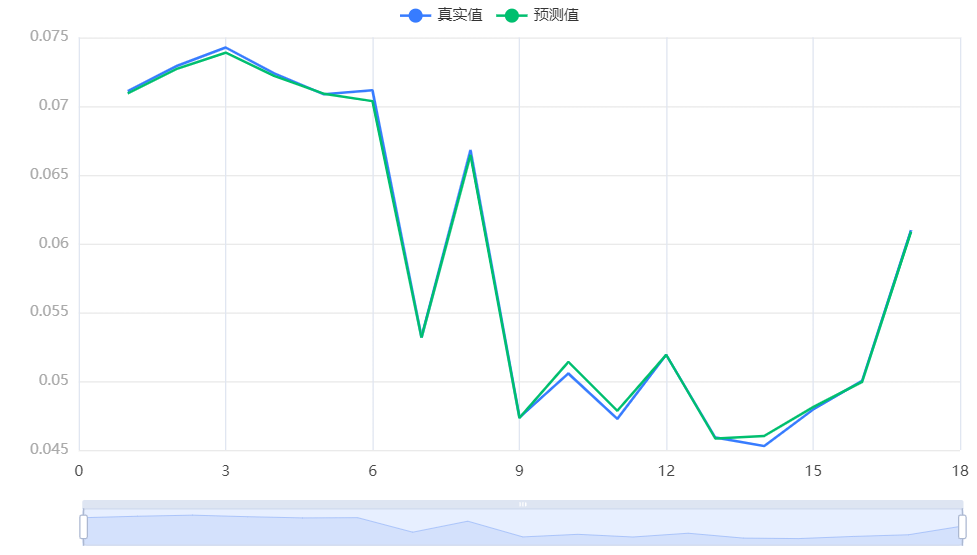
\includegraphics[width=0.9\textwidth]{img/效果比对图.png} % 图片相对位置 
	\caption{效果比对图} % 图片标题 
	\label{fig:figure 6} % 图片标签
\end{figure}

发现其预测值和真实值的曲线拟合虽然存在一些折点,但大体上拟合得十分优秀,与预期结果基本一致。

\textbf{Step4:对已风化的数据进行未风化时的成分预测}

提取表2的全部已风化的高钾玻璃样品的数据,联立15条回归方程,得到如下表所示的高钾玻璃未风化前的预测数据。
\begin{table}[H]
    \centering
	\caption{高钾玻璃风化前预测结果}
    \begin{tabular}{|c|c|c|c|c|c|c|}
    \hline
        文物采样点 & 07 & 09 & 10 & 12 & 22 & 27 \\ \hline
        $x_1$ & 92.63 & 95.02 & 96.77 & 94.29 & 92.35 & 92.72 \\ \hline
        $x_2$ & 0.033597712 & 0.020205613 & 0.015790981 & 0.038818306 & 0 & 0.101122203 \\ \hline
        $x_3$ & 0.042751476 & 0.59 & 0.92 & 1.01 & 0.74 & 0.183068383 \\ \hline
        $x_4$ & 1.07 & 0.62 & 0.21 & 0.72 & 1.66 & 0.94 \\ \hline
        $x_5$ & 0.006068596 & 0.005403809 & 0.003871925 & 0.010528593 & 0.64 & 0.54 \\ \hline
        $x_6$ & 1.98 & 1.32 & 0.81 & 1.46 & 3.5 & 2.51 \\ \hline
        $x_7$ & 0.17 & 0.32 & 0.26 & 0.29 & 0.35 & 0.2 \\ \hline
        $x_8$ & 3.24 & 1.55 & 0.84 & 1.65 & 0.55 & 1.54 \\ \hline
        $x_9$ & 0.09414252 & 0.080138485 & 0.071838606 & 0.161502668 & 0 & 0.395733507 \\ \hline
        $x_{10}$ & 0.067232087 & 0.073653143 & 0.057291679 & 0.118609805 & 0 & 0.261893897 \\ \hline
        $x_{11}$ & 0.61 & 0.35 & 0.001724109 & 0.15 & 0.21 & 0.36 \\ \hline
        $x_{12}$ & 0.001306109 & 0.001553981 & 0.001367797 & 0.003337039 & 0 & 0.005424483 \\ \hline
        $x_{13}$ & 0.007037408 & 0.005505709 & 0.003911147 & 0.011114358 & 0 & 0.029802936 \\ \hline
        $x_{14}$ & 0.047864091 & 0.04353926 & 0.034203756 & 0.086089231 & 0 & 0.212954589 \\ \hline
        $x_{15}$ & 风化 & 风化 & 风化 & 风化 & 风化 & 风化 \\ \hline
        总和 & 100 & 100 & 100 & 100 & 100 & 100 \\ \hline
    \end{tabular}
\end{table}

与上述步骤类似,提取已风化的铅钡玻璃数据代入铅钡玻璃联立方程中得到如下表所示的部分预测结果。
对于其余未展示的预测结果详见附录。

\begin{table}[H]
    \centering
	\caption{铅钡玻璃风化前预测结果}
    \begin{tabular}{|c|c|c|c|c|c|}
    \hline
        文物采样点 & 2 & 8 & 08严重风化点 & 11 & 19  \\ \hline
        $x_1$ & 36.28 & 20.14 & 4.61 & 33.59 & 29.64  \\ \hline
		$x_2$ & 0.020015895 & 0.127769334 & 1.257192536 & 0.888276262 & 0.374655333 \\ \hline
        $x_3$ & 1.05 & 0.007344282 & 0.083634612 & 0.21 & 0.053429852  \\ \hline
        $x_4$ & 2.34 & 1.48 & 3.19 & 3.51 & 2.93 \\ \hline
        $x_5$ & 1.18 & 0.01732933 & 0.162292009 & 0.71 & 0.59 \\ \hline
        $x_6$ & 5.73 & 1.34 & 1.11 & 2.69 & 3.57 \\ \hline
        $x_7$ & 1.86 & 0.013572252 & 0.130624745 & 0.12366741 & 1.33 \\ \hline
        $x_8$ & 0.26 & 10.41 & 3.14 & 4.93 & 3.51 \\ \hline
        $x_9$ & 47.43 & 28.68 & 32.45 & 25.39 & 42.82  \\ \hline
        $x_{10}$ & 0.057665039 & 31.23 & 30.62 & 14.61 & 5.35 \\ \hline
        $x_{11}$ & 3.57 & 3.59 & 7.56 & 9.38 & 8.83  \\ \hline
        $x_{12}$ & 0.19 & 0.37 & 0.53 & 0.37 & 0.19 \\ \hline
		$x_{13}$ & 0.003644047 & 0.013984802 & 0.126256097 & 0.07711458 & 0.055316838  \\ \hline
        $x_{14}$ & 0.028675018 & 2.58 & 15.03 & 0.910941748 & 0.756597977  \\ \hline
        总和 & 100 & 100 & 100 & 97.39 & 100 \\ \hline
    \end{tabular}
\end{table}









%第六部分
\section{问题二的模型建立与求解}
\subsection{问题分析}
本问又是可以细分为三小问,仍然是对数据的规律性和划分做分析处理。我们引入生物类别划分之间的"亚种"这一概念来解释本问中所提的亚类。存在一物种$A$以及物种$B$
,$B$由$A$变异而来,二者已经有了基因上的差别,但存在种群$a$来源于$A$,在环境的改变下逐渐演化,想$B$靠拢,但仍划分于$A$,这一种群就可成为亚种。
依据题目我们给出不同玻璃类型之间的未风化的样品会存在不同的亚类,在向风化靠拢,因为最终风化是必然性,划分的刻度就是趋向于风化的程度。
考虑到数据存在多重共线性问题(问题一已证)以及亚类划分的复杂,我们在本问采用$K-means++$—$BP$神经网络混合模型来进行对亚类的划分。无监督聚类后经过过采样处理
利用$BP$神经网络进行训练分类。具体思路的流程图如下:

\begin{figure}[H]\centering
	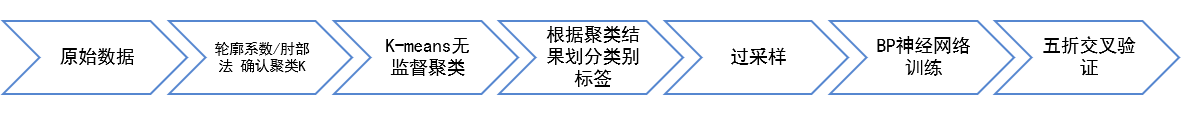
\includegraphics[width=0.9\textwidth]{img/第二问流程图.png} % 图片相对位置 
	\caption{求解玻璃制品亚分类流程图} % 图片标题 
	\label{fig:figure 6} % 图片标签
\end{figure}

\subsection{模型选择}
% \subsubsection{集成学习模型}
% 由于数据集的有限性,要深入探玻璃制品的分类规律,我们借助了集成学习的来进行分类规律的分析和预测。集成学习方法是一项强大的技术,它通过组合多个模型的输出来生成最终预测 [146]。集成学习时,重采样集成技术被广泛使用,已成功解决许多不同应用中的不均衡数据集问题。选择并使用一组准确且多样化的集成成员时,可以提高最终集成性能与泛化能力[55]。




\subsubsection{K-means++}
要探究对不同类别的玻璃制品对不同的化学成分进行亚分类,常见的聚类方法有$K-means$和层次聚类,两种模型相比之下前者的能够处理大量的数据,后者往往是计算样本之间
的距离,合并距离近的两对样本,再计算再合并,在时间复杂度上较大,处理大量数据时的效果不佳。同时$K-means$在聚类中心点的选择上会随机选择最小值或最大值,对算法影响
较大。$K-means++$在初始值的处理上就比$K-means$更好,降低了对算法和结果的分类的影响。

但由于我们的数据集不是很多,在聚类分析中的距离计算上,可能会有一些聚类的结果偏差较大,为了提高划分的准确性,采用$K-means++$和$BP$神经网络的混合模型,在聚类后对所得的
标签值经过$BP$神经网络的训练和检验,来划分结果。

本文原本先采用主成分分析法对化学成分指标进行降维处理,希望得到更加有用的数据,所得主成分为七组,通过肘部法所确定的建议聚类类别也为七类,我们认为其对最终
的聚类无实质性的作用,这七个主成分因子会对最终的分类结果产生较强的干扰,故本问中不进行主成分分析。


% \subsection{集成学习模型建立}
% 搭建一个目标集成算法包括几个分类任务,每一个都由一个数据集、一个诱导器和一个分类器组成[145]。构建预测模型的集成分三步:成员生成、成员选择和成员组合。
% 首先,是建立多样化的基础模型;
% 其次,成员选择,是一个可选步骤,它使用启发式方法来修剪模型池;
% 最后,成员组合,负责通过组合其预测来生成一个集成的最终输出。

% \subsubsection{投票机制}
% 集成学习策略应始终提供准确和多样化模型之间的权衡,这通过误差-歧义分解进行总结。这意味着集成的泛化误差是由所有个人错误和歧义,可以尝试通过减少泛化误差和增加每个个体的模糊性来减少整体泛化误差。我们考虑采用加权平均的方法来处理集合,集合的每个候选模型的最佳权重可以通过进化成员组合获得。据此,我们根据模型的基本模型在数据集上的表现进行加权,执行加权多数投票方案,以此优化分类结果。权重分配公式如下:

% \begin{equation}
% 	W_i = \frac{A_i}{\sum_{i=1}^7 A_i}
% \end{equation}

% \subsubsection{分类器建立}

% 本问所选择的基分类器为:$LGBMClassifier$, $LogisticRegression$, $AdaBoostClassifier$, $Stac$  \\
% $kingClassifier$, $RandomForestClassifier$,$SVC$,$GradientBoostingClassifier$。涉及的分类器具体有两种,
% 一类为$LogisticRegression$和$SVC$的基本学习算法,$SVC$用作元分类器,对上一级的预测结果进行纠错。

% \textbf{1.}$LogisticRegression$是一种用于解决二分类(0-1)问题的机器学习方法,用于估计某种事物的可能性。回归模型定义如下:
% \begin{equation}
% 	logit (p) = \ln (\frac{p}{1-p})
% \end{equation}

% 即:$p = \frac{1}{1+e^{-logit (p)}}$,通过极大似然估计来求解参数,将结果汇聚到(0,1)之间,在传统的预测评估的问题中
% 其准确率往往较高。

% 而$AdaBoostClassifier$、$GradientBoostingClassifier$、$RandomForestClassifier$都是增强机器学习算法的分类器,具有很强的泛化能力。

% \textbf{2.}$AdaBoostClassifier$算法是对所有的训练样本进行赋权,训练出一个合理的基分类器,后进行迭代$n$次,每次迭代都会修改出错的样本权重,最终组合成一个综合分类器。

% \textbf{3.}$GradientBoostingClassifier$需要输入数据集$S$和损失函数$L(y_i,F(x))$,损失函数一般选择交叉熵:
% \begin{equation}
% 	L(y_i,F(x)) = -[\sum_{i=1}^N y_i \log (p)+(1-y_i) \log (1-p)]
% \end{equation}

% 其中$y$是标签,$p$是预测的概率。

% 最终转化为:
% \begin{equation}
% 	L(y_i,F(x)) = -y_i \log (odds)+\log (1+e^{\log (odds)})
% \end{equation}


% 函数确立后即可建立初始值$F_0(x) = argmin_\gamma \sum _{i=1}^n L(y_i,\gamma)$,然后开始从第0棵树进行迭代,依次计算出概率,拟合成一颗回归树,分别得到叶子节点。

% \textbf{4.}$RandomForestClassifier$就是随机森林,其通过大量的决策树进行搭建,不同的决策树会通过投票机制来做出分类,最后汇聚到森林尽头结合形成一个最终的分类结果,优于任何一个决策树的独立结果。

%  \subsubsection{模型集成和$Exhaustive search$寻优}

%  使用$StackingCVClassifier$进行模型集成,并且设置五折交叉验证进行泛化能力的评估,最终器分类结构如下:

%  \begin{figure}[H]\centering
%      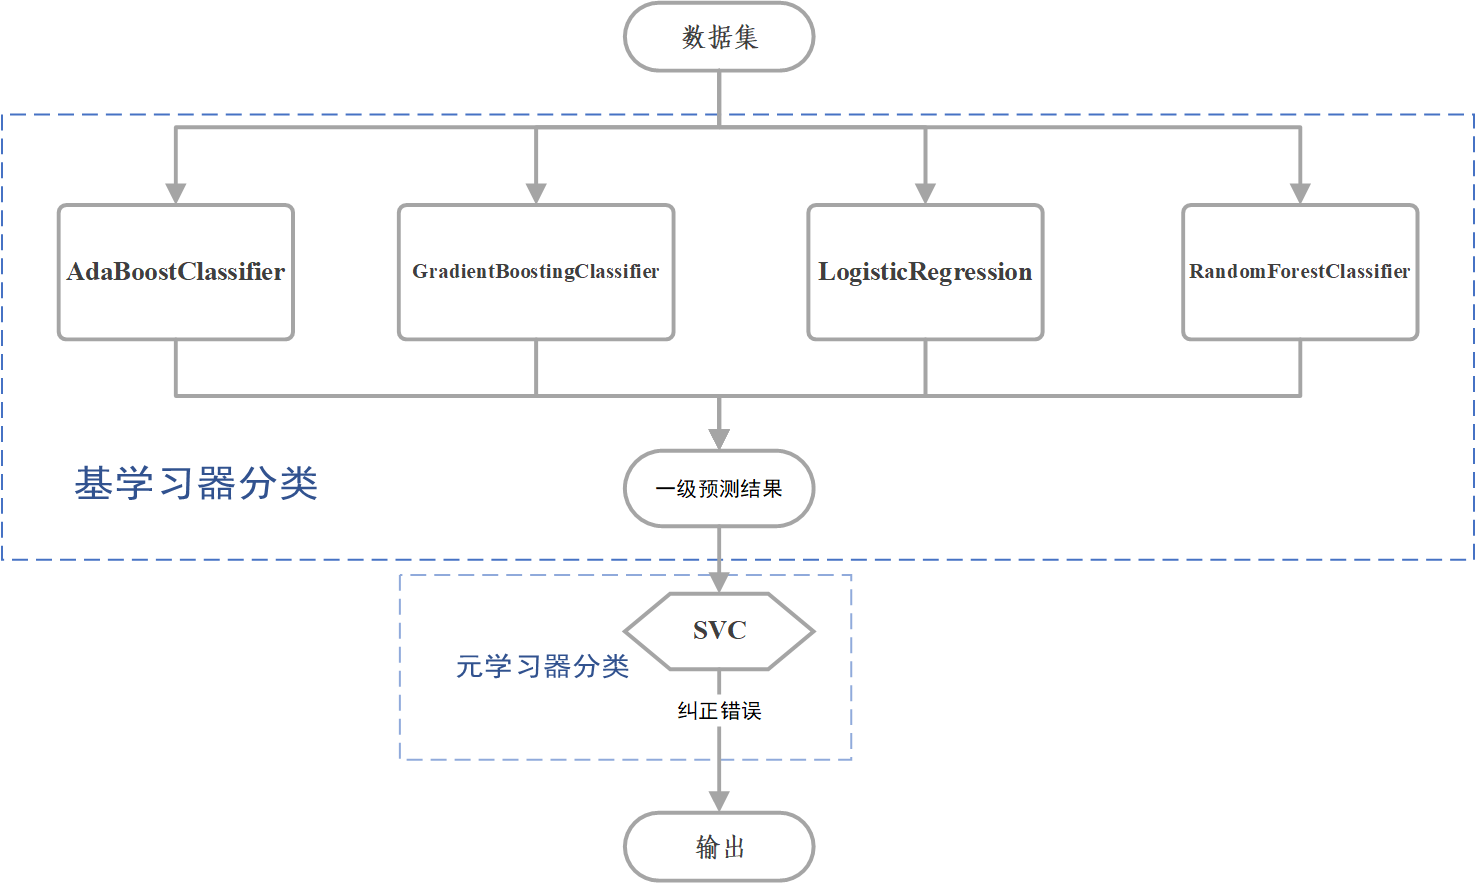
\includegraphics[width=0.9\textwidth]{img/器分类结构.png} % 图片相对位置 
%      \caption{器分类结构} % 图片标题 
%      \label{fig:figure 9} % 图片标签
%  \end{figure}

%  通过穷举来寻优,依次按照树的结构去搜索,常见的有$DFS$和$BFS$,区别在于广度搜索还是深度搜索,在本问中,数据集不大的情况下使用$Exhaustive search$来进行寻优的时间复杂度不大,有着合理性,可以通过对树的搜索遍历来找到最优的分类结果。








\subsection{K-means++模型建立}
\subsubsection{肘部法和轮廓系数法确定$K$}
\textbf{1.肘部法}

设样本簇群为$Q$,簇为$Q_i$, $q$为$Q_i$的样本点,$Q_i$均值为$\bar{Q_i}$,则可得肘部法的指标公式为:
\begin{equation}
	erro = \sum _{i=1} ^K \sum\left\lvert p-\bar{Q_i} \right\rvert ^2
\end{equation}

随着$K$的增大,聚合程度会越来越高,$erro$也会越来越小,变化率不断增大,当到达一个理想的值,变化率会缓慢下降,直到
趋于平缓,这一理想值就是所要求的$K$。如下为肘部法所计算出高钾类和铅钡类的情况。

\begin{figure}[htbp]
    \centering
    \subfigure[铅钡]{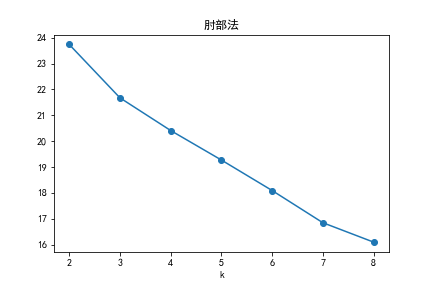
\includegraphics[height=5.7cm,width=7.5cm]{img/肘部法_铅钡.png}}
    \subfigure[高钾]{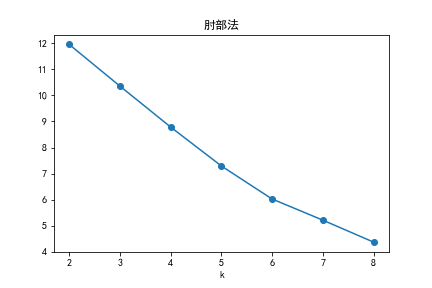
\includegraphics[height=5.7cm,width=7.5cm]{img/肘部法_高钾.png}}
    \caption{肘部法}
    \label{fig}
\end{figure}

观测可得肘部法变化不明显,找不到转折突变值,于是采用轮廓系数法来进行估计。

\textbf{2.轮廓系数法}

轮廓系数法的原理是选择使系数较大所对应的$K$值。分别计算样本与同簇样本和异簇样本之间的平均距离,
以均值来分别代表其不相似度$a_i$和$b_i$。得到轮廓系数为$e_i = \frac{b_i-a_i}{max(a_i,b_i)}$。
通过计算得到如下结果:

\begin{figure}[H]
    \centering
    \subfigure[铅钡]{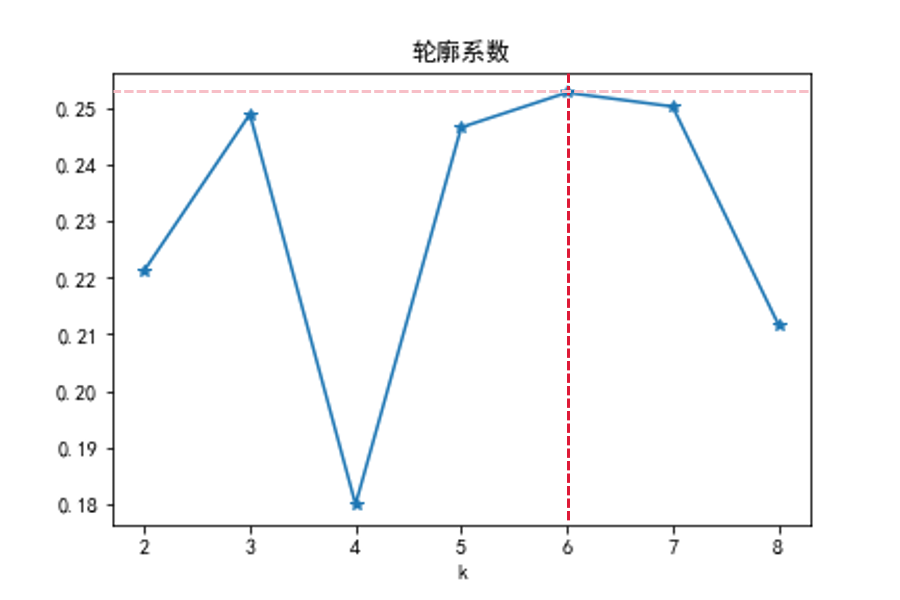
\includegraphics[height=5.7cm,width=7.5cm]{img/轮廓系数_铅钡_label.png}}
    \subfigure[高钾]{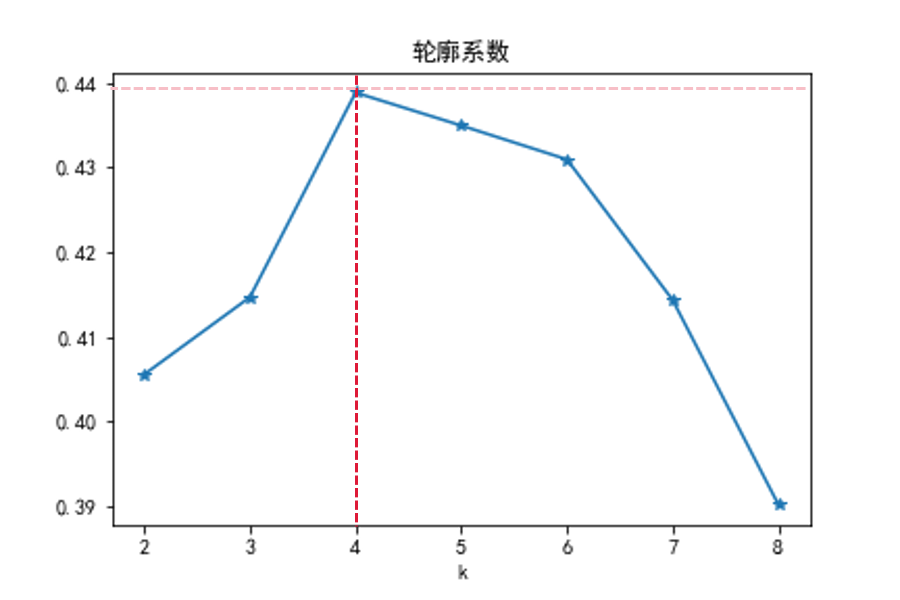
\includegraphics[height=5.7cm,width=7.5cm]{img/轮廓系数_高钾_label.png}}
    \caption{轮廓系数法}
    \label{fig}
\end{figure}

最终选取高钾的簇个数$K$为4,铅钡的的簇个数$K$为6。

\subsubsection{K-means++聚类}
通过$K-means++$聚类得到高钾和铅钡两组结果如下:
\begin{figure}[H]
    \centering
    \subfigure[铅钡]{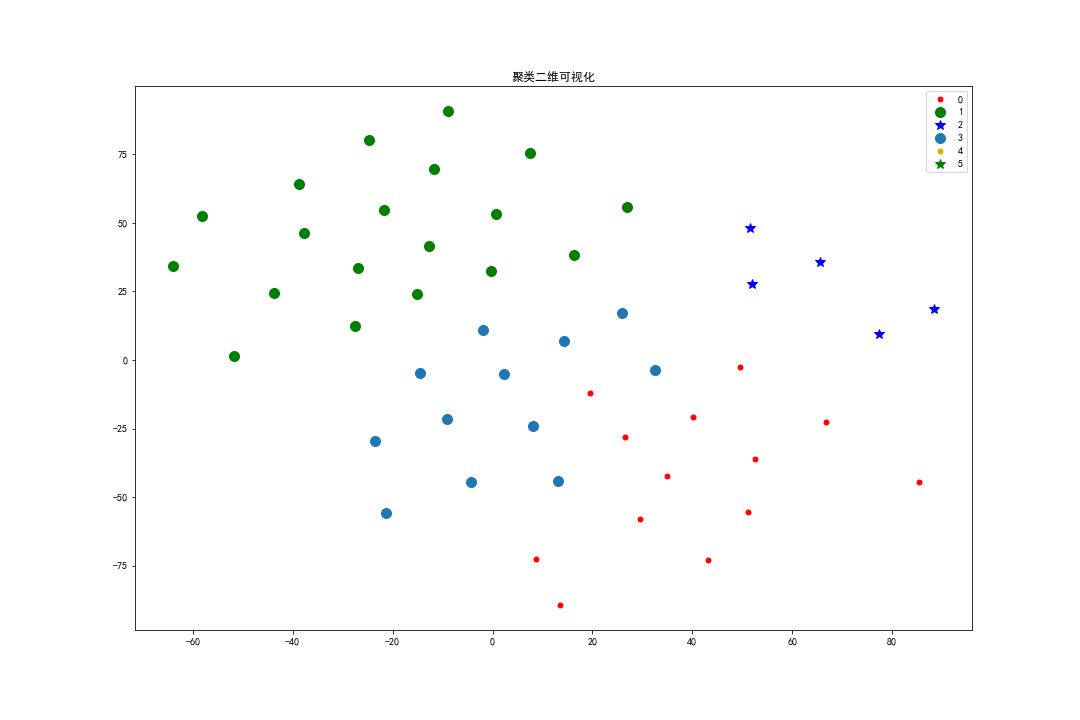
\includegraphics[height=5.7cm,width=7.7cm]{img/k-means_铅钡.png}}
    \subfigure[高钾]{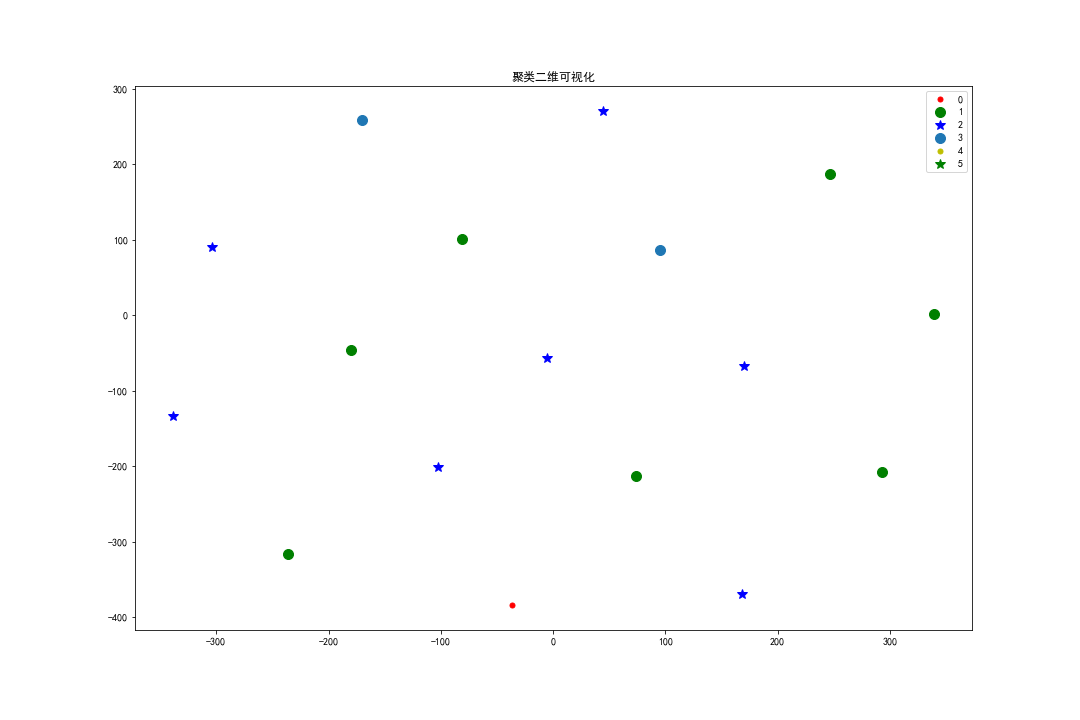
\includegraphics[height=5.7cm,width=7.7cm]{img/k-means_高钾.png}}
    \caption{轮廓系数法}
    \label{fig}
\end{figure}

根据聚类图分析,铅钡和高钾分别分为了四类和六类,但有的点之间的距离较远,分类的效果仍不是很好。

\subsubsection{$BP$神经网络训练}

将$K-means++$划分的聚类结果作为类别标签,输入BP神经网络进行训练。我们使用遗传算法作为启发式算法进行模型超参寻优。
遗传算法是对全局随机搜索优化,从任一点出发,一直搜索,随着时间变化会逐渐找到最优解。我们认为遗传算法结合$BP$神经网络
能够训练出更准确的训练模型,用来分类的效果更好。

\subsection{模型求解}

\textbf{Step1:}交叉评估

为了避免由于数据集划分不合理而导致的在训练集上过拟合问题,我们使用5折交叉验证将数据集划分为5个大小相似的互斥子集,
每次用4个子集的并集作为训练集,剩下的那一个子集作测试集,进行5次训练和测试,最后得到5个评估结果的均值。
故此交叉验证得到评估结果才能跟好的评估模型的泛化性。流程图如下:

\begin{figure}[H]\centering
	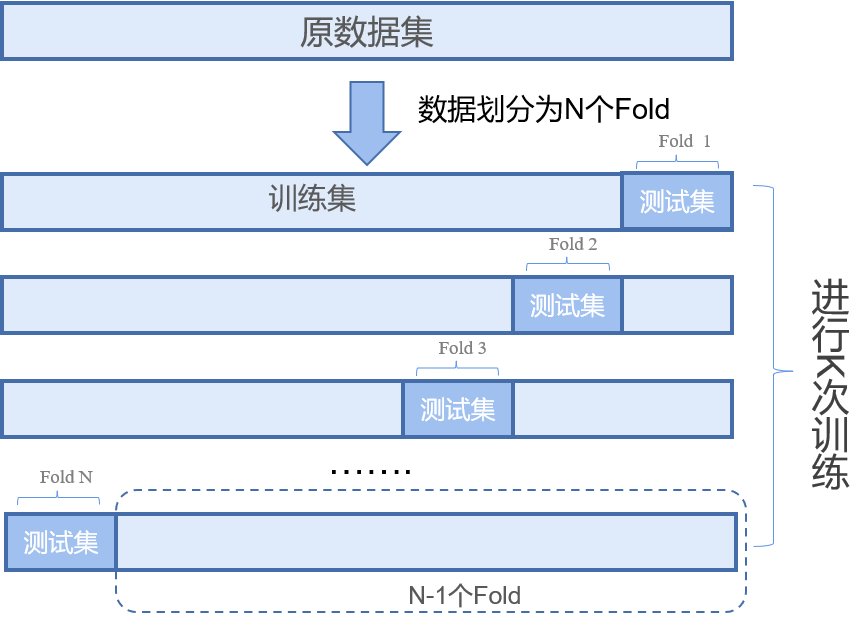
\includegraphics[width=0.69\textwidth,height=0.6\textwidth]{img/交叉评估流程图.png} % 图片相对位置 
	\caption{交叉评估流程图} % 图片标题 
	\label{fig:figure 6} % 图片标签
\end{figure}

\textbf{Step2:}随机采样处理

经观察发现$BP$训练铅钡类型的数据集时的模型表现效果较差,通过统计发现类别标签不均衡,于是采用随机采样策略进行处理。
即设类别最多的个数为样本采样上限,在其他类别中对其求均值后扩展到采样上限。

\textbf{Step3:}遗传算法寻优

在进行$BP$训练时,混合遗传算法进行寻优,合理的调参,得出以下最优的参数:

\begin{table}[H]                                                                                                     
    \centering
    \caption{最优参数列表}
    \begin{tabular}{|l|l|l|}
    \hline
        参数名 & BP(高钾) & BP(铅钡) \\ \hline
        训练用时 & 0.306s & 0.454s \\ \hline
        数据切分 & 0.8 & 0.8 \\ \hline
        数据洗牌 & 是 & 是 \\ \hline
        交叉验证 & 5 & 5 \\ \hline
        激活函数 & relu & relu \\ \hline
        求解器 & adam & adam \\ \hline                                       
        学习率 & 0.01 & 0.01 \\ \hline
        L2正则项 & 0.1 & 0.1 \\ \hline
        迭代次数 & 400 & 400 \\ \hline
        隐藏第1层神经元数量 & 10 & 10 \\ \hline
    \end{tabular}
\end{table}

\textbf{Step4:}最后进行模型的评估



分别对高钾类型和铅钡类型的模型进行评估其得分:

\begin{table}[H]
    \centering
    \caption{模型评估}
    \begin{tabular}{|l|l|l|l|l|}
    \hline
        高钾 & 准确率 & 召回率 & 精确率 & F1 \\ \hline
        训练集 & 1 & 1 & 1 & 1 \\ \hline
        交叉验证集 & 1 & 1 & 1 & 1 \\ \hline
        测试集 & 1 & 1 & 1 & 1 \\ \hline
        ~ & ~ & ~ & ~ & ~ \\ \hline
        铅钡 & ~ & ~ & ~ & ~ \\ \hline
        训练集 & 1 & 1 & 1 & 1 \\ \hline
        交叉验证集 & 0.95 & 0.95 & 0.925 & 0.933 \\ \hline
        测试集 & 1 & 1 & 1 & 1 \\ \hline
    \end{tabular}
\end{table}


\subsubsection{敏感度分析}
使用python中的Salib进行敏感度分析,我们计算原本数据集中每个特征的最大值和最小值作为边界,进而采样生成32000个特征向量进行预测,最后根据预测结果进行敏感度评估计算。

通过以下三个指标进行分析:

    1.一阶敏感度$S1$:度量单变量输入对输出方差的影响贡献度
         
    2.二阶敏感度$S2$:度量两个变量输入相互作用对输出方差的贡献
    		
    3.总阶敏感度$ST$:度量模型输入对输出方差的贡献,在一阶,二阶乃至更高阶都有计算




% \left\{
% \begin{array}{l}
% 一阶敏感度S1:度量单变量输入对输出方差的影响贡献度      \\
% 二阶敏感度S2:度量两个变量输入相互作用对输出方差的贡献		\\
% 总阶敏感度ST:度量模型输入对输出方差的贡献,在一阶,二阶乃至更高阶都有计算
% \end{array} \right

一阶灵敏度表示由输入的一个参数变化引起的目标变量方差变化的比例。总阶指数表示给定参数的目标变量中的总方差,包括由其与任何其他输入变量的任何阶的相互作用引起的所有方差。

下图为一阶灵敏度$S1$与$ST$在各个成分上的对比,通过柱状图分析,我们可以明显观察到可以看到,成分$SiO_2$和成分$Na_2O$都表现出了一阶灵敏性,成分$K_2O$还出现的了负数的情况,是由于样本数量较少,存在抽样误差,导致指标为负数。
\begin{figure}[H]\centering
	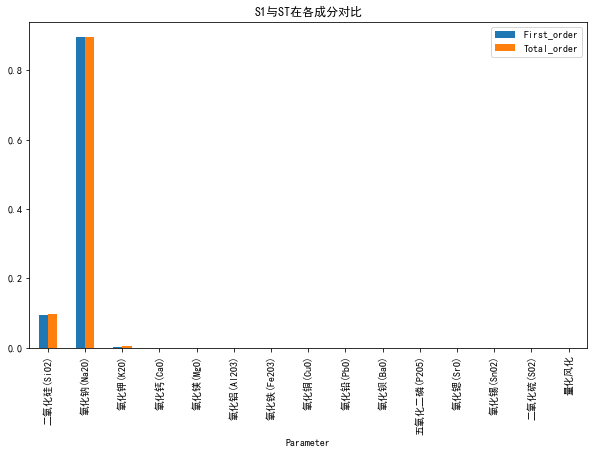
\includegraphics[width=1\textwidth,height=0.7\textwidth]{img/S1.png} % 图片相对位置 
	\caption{第二问一阶灵敏度分析} % 图片标题 
	\label{fig:figure 6} % 图片标签
\end{figure}

计算$SiO_2,Na_2O,K_2O$之间的交互作用:

% \left\{
% \begin{array}{rcl}
% SiO_2-Na_2O = -0.006480232647261386      \\
% SiO_2-K_2O =	0.0010737091488327733		\\
% Na_2O-K_2O =0.0020852247605257102
% \end{array} \right.

\[\left\{\begin{array}{llcl}
    SiO_2-Na_2O = -0.006480232647261386      \\
    SiO_2-K_2O =	0.0010737091488327733		\\
    Na_2O-K_2O =0.0020852247605257102
\end{array} \right.\]


$SiO_2-Na_2O$的指数都小于0,说明随着样本数量的增加,它们的误差会不断减小。$SiO_2-K_2O$以及$Na_2O-K_2O$的指标为正,说明两者之间具有较强的关联性,会出现计算误差。

二阶灵敏度表示处理两个参数组合下的灵敏度变换,故此通过热力图进行可视化分析,我们可以发现二阶交互作用很小,所有指数的值都小于0.02,成分$Na_2O$的二阶灵敏度最高。

\begin{figure}[H]\centering
	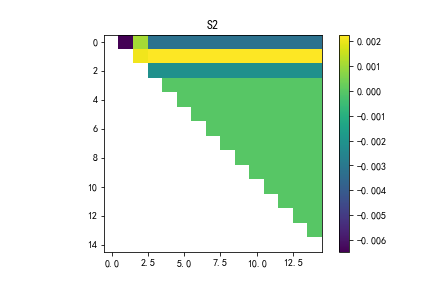
\includegraphics[width=1\textwidth,height=0.6\textwidth]{img/S2_heatmap.png} % 图片相对位置 
	\caption{第二问二阶灵敏度分析} % 图片标题 
	\label{fig:figure 6} % 图片标签
\end{figure}


%第七部分
\section{问题三的模型建立与求解}
\subsection{问题分析}
问题三要求我们对附录表单三中的样品数据进行鉴别其玻璃所属的类型。过程需要分析其化学成分的数据后
再对类别进行鉴别预测,可将其转化为一个集成学习经过数据集训练后对目标数据进行预测的问题。
首先对数据缺失值进行填补,结合表单二进行模型训练和补充后对一些定类数据处理为定量数据。其次使用集成模型,集成多个成员模型,通过$Exhaustive search$对其寻优,利用
划分好的数据集进行模型的训练,得出良好的预测模型然后再对目标数据进行预测。具体流程图如下:


\begin{figure}[H]\centering
	
\includegraphics[width=0.9\textwidth]{img/第三问流程图.png} % 图片相对位置 
	\caption{对未知类型玻璃分类流程图} % 图片标题 
	\label{fig:figure 7} % 图片标签
\end{figure}

\subsection{基于随机森林的数据填补}
附录表单三给出的样本数据存在着一些空白值,考虑测量误差的存在,我们仍决定采用第一问中所用到的随机森林算法来填补缺失值。

由于其数据量少,以及缺失值:无缺失值=33:54,缺失值占比高,故此,如果直接采用随机森林填补,训练出来的随机森林拟合度差,填补的缺失值可信度低。所以我们将填补后的表单二与包含缺失值的表单三进行关连,使用连表后的数据进行模型训练和填补,增加填补值的可靠性。其他的填补操作如同先前的随机森林的数据填补方式,下表是填补结果。

\begin{table}[H]
    \centering
	\caption{随机森林填补结果}
    \begin{tabular}{|l|l|l|l|l|l|l|l|l|}
		
    \hline
        文物采样点 & A1 & A2 & A3 & A4 & A5 & A6 & A7 & A8 \\ \hline
        $x_1$ & 78.45 & 37.75 & 31.95 & 35.47 & 64.29 & 93.17 & 90.83 & 51.12 \\ \hline
        $x_2$ & 0.03865 & 0.062002 & 0.373588 & 1.264156 & 1.2 & 0.2235 & 0.092727 & 0 \\ \hline
        $x_3$ & 0.409402 & 0.515894 & 1.36 & 0.79 & 0.37 & 1.35 & 0.98 & 0.23 \\ \hline
        $x_4$ & 6.08 & 7.63 & 7.19 & 2.89 & 1.64 & 0.64 & 1.12 & 0.89 \\ \hline
        $x_5$ & 1.86 & 0.089196 & 0.81 & 1.05 & 2.34 & 0.21 & 0.125788 & 0 \\ \hline
        $x_6$ & 7.23 & 2.33 & 2.93 & 7.07 & 12.75 & 1.52 & 5.06 & 2.12 \\ \hline
        $x_7$ & 2.15 & 0.346143 & 7.06 & 6.45 & 0.81 & 0.27 & 0.24 & 0 \\ \hline
        $x_8$ & 2.11 & 0.292707 & 0.21 & 0.96 & 0.94 & 1.73 & 1.17 & 9.01 \\ \hline
        $x_9 $& 0.020264 & 34.3 & 39.58 & 24.28 & 12.23 & 0.326278 & 0.059486 & 21.24 \\ \hline
        $x_{10}$ & 0.036171 & 0.55726 & 4.69 & 8.31 & 2.16 & 0.172133 & 0.058125 & 11.34 \\ \hline
        $x_{11}$ & 1.06 & 14.27 & 2.68 & 8.45 & 0.19 & 0.21 & 0.13 & 1.46 \\ \hline
        $x_{12}$ & 0.03 & 0.03702 & 0.52 & 0.28 & 0.21 & 0.004691 & 0.001063 & 0.31 \\ \hline
        $x_{13}$ & 0.015512 & 0.016618 & 0.212994 & 0.145549 & 0.49 & 0.05717 & 0.02281 & 0 \\ \hline
        $x_{14}$ & 0.51 & 0.083158 & 0.433418 & 0.590295 & 0.38 & 0.116229 & 0.11 & 2.26 \\ \hline
        $x_{15}$ & 0 & 1 & 0 & 0 & 1 & 1 & 1 & 0 \\ \hline
    \end{tabular}
\end{table}

最后将数据集进行划分,按照训练集:测试集=7:3的比例划分,并进行随机打乱处理。

\subsection{模型建立}
\subsubsection{集成模型的引入}
集成学习方法是一项强大的技术,它通过组合多个模型的输出来生成最终预测 \cite{ref3} 。集成学习时,重采样集成技术被广泛使用,已成功解决许多不同应用中的不均衡数据集问题。选择并使用一组准确且多样化的集成成员时,可以提高最终集成性能与泛化能力\cite{ref4} 。

搭建一个目标集成算法包括几个分类任务,每一个都由一个数据集、一个诱导器和一个分类器组成。构建预测模型的集成分三步:成员生成、成员选择和成员组合。
首先,是建立多样化的基础模型;
其次,成员选择,是一个可选步骤,它使用启发式方法来修剪模型池;
最后,成员组合,负责通过组合其预测来生成一个集成的最终输出。


可表述为一个优化问题。我们旨在通过创建候选模型池来挑选最终用于集成的模型,使用$Exhau$ \\ $stive search$进行模型寻优,候选模型的预测分数和复杂度值是最重要的评估标准,模型的训练以及筛选过程如图:

\begin{figure}[H]\centering
	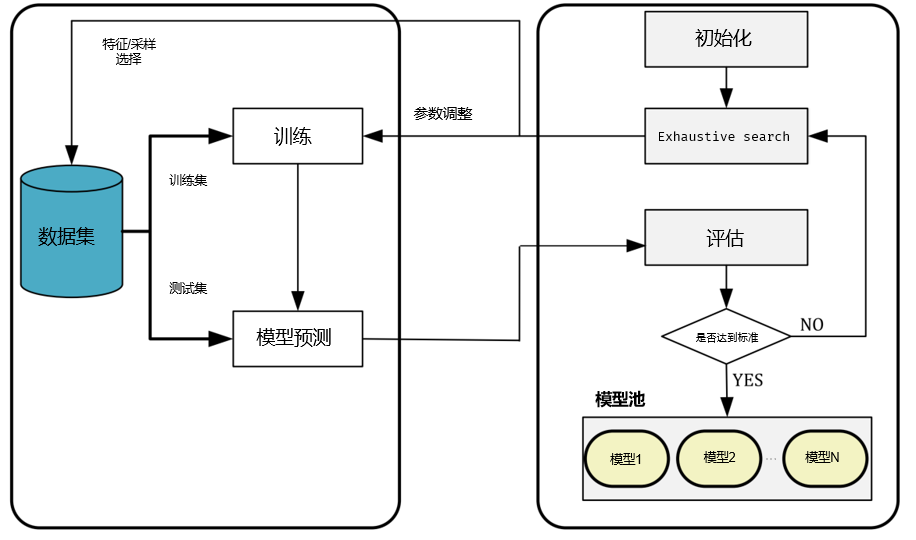
\includegraphics[width=0.9\textwidth]{img/集成模型流程.png} % 图片相对位置 
	\caption{集成模型流程} % 图片标题 
	\label{fig:figure 8} % 图片标签
\end{figure}

\subsubsection{集成模型建立}
投票法是一种遵循少数服从多数原则的集成学习模型,使用投票法可以集成多个模型进而降低方差,提高模型的鲁棒性,在理想情况下,投票法的预测效果应当优于其中任何一个基模型的预测效果。根据实验对比,我们最终使用软投票进行预测。

集成学习策略应始终提供准确和多样化模型之间的权衡,这通过误差-歧义分解进行总结。这意味着集成的泛化误差是由所有个人错误和歧义,可以尝试通过减少泛化误差和增加每个个体的模糊性来减少整体泛化误差。我们考虑采用加权平均的方法来处理集合,集合的每个候选模型的最佳权重可以通过进化成员组合获得。据此,我们根据模型的基本模型在数据集上的表现进行加权,执行加权多数投票方案,以此优化分类结果。权重分配公式如下:

\begin{equation}
	W_i = \frac{A_i}{\sum_{i=1}^7 A_i}
\end{equation}

通过数据分析,我们发现高钾:铅钡的样本数量比约为1:3,在合理比率之内,所以我们认为不存在轻微的类别不平衡问题。由于,集成学习需要多样性的分类器,故此我们使用进化采样的方式来缓解类别不平衡问题。进化采样和集成方法允许拟合函数促进过采样或欠采样数据集的多样性,从而在处理不平衡的数据集时可以得到更准确的结果。

\textbf{Step1:}分类器建立

本问所选择的基分类器为:$LGBMClassifier$, $LogisticRegression$, $AdaBoostClassifier$, $Stac$  \\
$kingClassifier$, $RandomForestClassifier$,$SVC$,$GradientBoostingClassifier$。涉及的分类器具体有两种,
一类为$LogisticRegression$和$SVC$的基本学习算法,$SVC$用作元分类器,对上一级的预测结果进行纠错。

\textbf{1.}$LogisticRegression$是一种用于解决二分类(0-1)问题的机器学习方法,用于估计某种事物的可能性。回归模型定义如下:
\begin{equation}
	logit (p) = \ln (\frac{p}{1-p})
\end{equation}

即:$p = \frac{1}{1+e^{-logit (p)}}$,通过极大似然估计来求解参数,将结果汇聚到(0,1)之间,在传统的预测评估的问题中
其准确率往往较高。

而$AdaBoostClassifier$、$GradientBoostingClassifier$、$RandomForestClassifier$都是增强机器学习算法的分类器,具有很强的泛化能力。

\textbf{2.}$AdaBoostClassifier$算法是对所有的训练样本进行赋权,训练出一个合理的基分类器,后进行迭代$n$次,每次迭代都会修改出错的样本权重,最终组合成一个综合分类器。

\textbf{3.}$GradientBoostingClassifier$需要输入数据集$S$和损失函数$L(y_i,F(x))$,损失函数一般选择交叉熵:
\begin{equation}
	L(y_i,F(x)) = -[\sum_{i=1}^N y_i \log (p)+(1-y_i) \log (1-p)]
\end{equation}

其中$y$是标签,$p$是预测的概率。

最终转化为:
\begin{equation}
	L(y_i,F(x)) = -y_i \log (odds)+\log (1+e^{\log (odds)})
\end{equation}


函数确立后即可建立初始值$F_0(x) = argmin_\gamma \sum _{i=1}^n L(y_i,\gamma)$,然后开始从第0棵树进行迭代,依次计算出概率,拟合成一颗回归树,分别得到叶子节点。

 $RandomForestClassifier$就是随机森林,其通过大量的决策树进行搭建,不同的决策树会通过投票机制来做出分类,最后汇聚到森林尽头结合形成一个最终的分类结果,优于任何一个决策树的独立结果。

\textbf{Step2:}模型集成

使用$StackingCVClassifier$进行模型集成,并且设置五折交叉验证进行泛化能力的评估,最终器分类结构如下:

\begin{figure}[H]\centering
	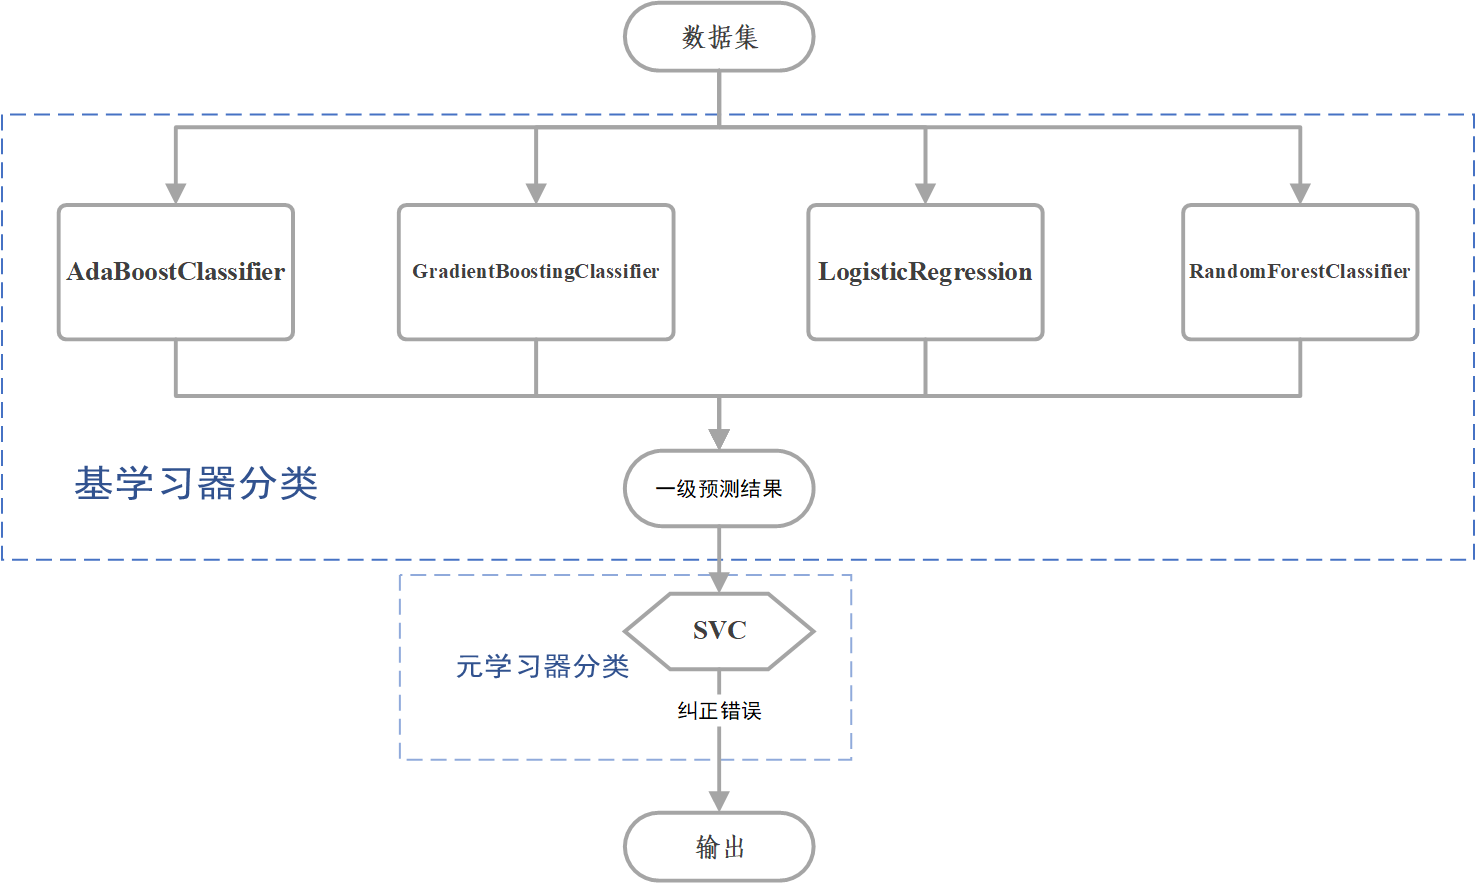
\includegraphics[width=0.9\textwidth]{img/器分类结构.png} % 图片相对位置 
	\caption{器分类结构} % 图片标题 
	\label{fig:figure 9} % 图片标签
\end{figure}

\textbf{Step3:} $Exhaustive search$寻优

通过穷举来寻优,依次按照树的结构去搜索,常见的有$DFS$和$BFS$,区别在于广度搜索还是深度搜索,在本问中,数据集不大的情况下使用$Exhaustive search$来进行寻优的时间复杂度不大,有着合理性,可以通过对树的搜索遍历来找到最优的分类结果。


\subsection{模型求解}

\textbf{Step1:}集成分类器拟合

对所采用的七个成员分类器进行数据的拟合和调参,通过$StackingCVClassifier$来选取最优参数,分别得出这些分类器的数据拟合结果如下:

\begin{table}[H]
    \centering
	\caption{分类器拟合结果}
    \begin{tabular}{|l|l|l|l|l|l|l|l|}
    \hline
        分类器 & LR & Ada & GDBT & SVC & RF & SC & LGBM \\ \hline
         综合准确率 & 1 & 1 & 1 & 1 & 1 & 1 & 0.984848 \\ \hline
        训练集准确率 & 1 & 1 & 1 & 1 & 1 & 1 & 1 \\ \hline
        测试集准确率 & 1 & 1 & 1 & 1 & 1 & 1 & 0.95 \\ \hline
        预测率 & 1 & 1 & 1 & 1 & 1 & 1 & 1 \\ \hline
        召回率 & 1 & 1 & 1 & 1 & 1 & 1 & 0.928571 \\ \hline
        AUC & 1 & 1 & 1 & 1 & 1 & 1 & 0.988095 \\ \hline
        f1 & 1 & 1 & 1 & 1 & 1 & 1 & 0.962963 \\ \hline
    \end{tabular}
\end{table}

据上表分析可得:搜索出上述模型符合该数据集的最优超参组合,通过验证后发现无论是训练集还是测试集的表现都十分良好,我们认为,之所以可以达到这么优秀的拟合效果,离不开最初的随机森林填补策略以及参数调优。

\textbf{Step2:}软投票结果

单纯看准确率来判断分类模型的结果是不够严谨的,此问加入了$AUC$值进行参考,通过观测$AUC$和$ROC$的曲线覆盖面积可以综合其他多种指标,$AUC$值一般>0.8则认为模型可接受。

虽然选择的七个分类器的效果都较为完美,但我们考虑到可能是数据集规模较小所导致。在预测其他的数据依然具有很大的不稳定性,单模型易受到干扰或者噪声的影响,较为敏感。
为了提高模型的泛化能力,降低噪声导致的预测错误,我们使用上述七个模型进行软投票分类,采用公式$W_i = \frac{A_i}{\sum_{i=1}^7 A_i}$进行加权投票,最终形成的$VoteModel$模型
在数据集上的表现依然呈现完美。结果如下表所示:

\begin{table}[H]
    \centering
	\caption{VoteModel拟合结果}
    \begin{tabular}{|l|l|l|l|l|l|l|l|}
    \hline
        分类器 &  综合准确率 & 训练集准确率 & 测试集准确率 & 预测率 & 召回率 & AUC & f1 \\ \hline
        VoteModel & 1 & 1 & 1 & 1 & 1 & 1 & 1 \\ \hline
    \end{tabular}
\end{table}

下图为$VoteModel$模型的$AUC$和$ROC$曲线覆盖图:

\begin{figure}[H]\centering
	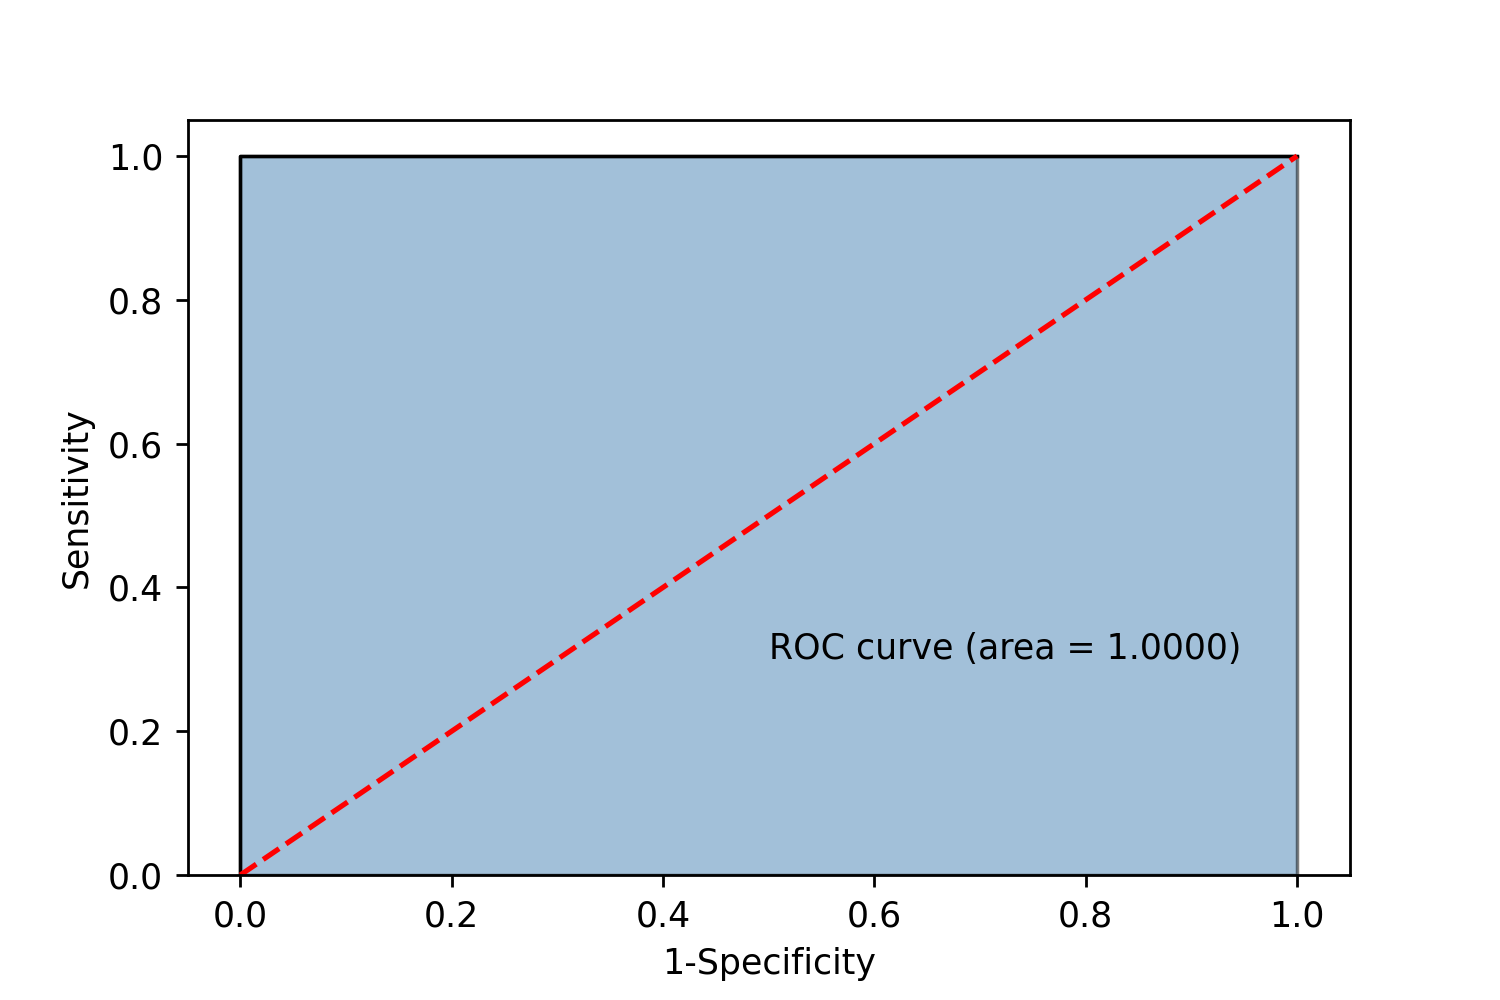
\includegraphics[width=0.9\textwidth]{img/AUC.png} % 图片相对位置 
	\caption{AUC和ROC曲线覆盖图} % 图片标题 
	\label{fig:figure 10} % 图片标签
\end{figure}

据图分析可发现其值为1.0,效果十分优秀。
\textbf{Step3:}提高模型的泛化能力

我们为了提高模型的泛化能力、模型拟合效果以及缓解数据集少导致模型敏感性提高的问题。我们使用所有的数据进行训练后的集成模型$VoteModel$对表单3进行预测,预测结果如下表所示:

\begin{table}[H]
    \centering
	\caption{鉴别结果}
    \begin{tabular}{|l|l|l|l|}
    \hline
        文物采样点 & 类型 & 高钾概率的置信度 & 铅钡概率的置信度 \\ \hline
        A1 & 高钾 & 0.846815 & 0.153185 \\ \hline
        A2 & 铅钡 & 0.120949 & 0.879051 \\ \hline
        A3 & 铅钡 & 0.081817 & 0.918183 \\ \hline
        A4 & 铅钡 & 0.077011 & 0.922989 \\ \hline
        A5 & 铅钡 & 0.133748 & 0.866252 \\ \hline
        A6 & 高钾 & 0.887034 & 0.112966 \\ \hline
        A7 & 高钾 & 0.877908 & 0.122092 \\ \hline
        A8 & 铅钡 & 0.109741 & 0.890259 \\ \hline
    \end{tabular}
\end{table}
据表分析得:模型对于正类的预测置信度高,说明最终设计的集成模型$VoteModel有$较好的泛化能力,对于给定的新数据分布表单3依然体现敏感性低的特点。

\subsection{敏感度分析}
\subsubsection{敏感度}
我们通过计算模型的预测情况来得到模型的SE敏感性,计算公式如下:
\begin{equation}
    SE=\frac{TP}{TP+FN}
\end{equation}

即通过计算正确预测为正的数目,在实际为正的总数目中的比例来衡量模型的敏感度,实际上评判的是模型的漏检率,SE越接近1,敏感度越低。

\subsubsection{特异性}
模型的误判率也是衡量模型能力的关键指标之一,对于特异性指标的计算公式如下:
\begin{equation}
    SP=\frac{TN}{TN+FP}
\end{equation}
即评判的是模型的误判率,SP越接近1,则认为模型的误判性越低。通过模型在测试集上的预测,计算对应的检测指标,得到$TP$,$FN$,$FP$,$TN$,进而得到$SE$以及$SP$,如下表:

\begin{table}[H]
    \centering
	\caption{$SE$和$SP$分析}
    \begin{tabular}{|l|l|l|}
    \hline
           & 实际为正 & 实际为负  \\ \hline
        预测为正(P) & 17(TP) &0(FP) \\ \hline
        预测为负(N) & 0(FN) &49(TN) \\ \hline
        % A1 & 高钾 & 0.846815 & 0.153185 \\ \hline
        % A2 & 铅钡 & 0.120949 & 0.879051 \\ \hline
        % A3 & 铅钡 & 0.081817 & 0.918183 \\ \hline
        % A4 & 铅钡 & 0.077011 & 0.922989 \\ \hline
        % A5 & 铅钡 & 0.133748 & 0.866252 \\ \hline
        % A6 & 高钾 & 0.887034 & 0.112966 \\ \hline
        % A7 & 高钾 & 0.877908 & 0.122092 \\ \hline
        % A8 & 铅钡 & 0.109741 & 0.890259 \\ \hline
    \end{tabular}
\end{table}

\begin{table}[H]
    \centering
	\caption{VoteModel分析结果}
    \begin{tabular}{|l|l|l|}
    \hline
         模型  & SE & SP  \\ \hline
        VoteModel & 1& 1 \\ \hline
    \end{tabular}
\end{table}
\subsubsection{敏感度分析}
下图为一阶灵敏度$S1$与$ST$在各个成分上的对比,通过柱状图分析,我们可以明显观察到可以看到,成分$SiO_2$和成分$Na_2O$都表现出了一阶灵敏性,成分$K_2O$还出现的了负数的情况,是由于样本数量较少,存在抽样误差,导致指标为负数。

\begin{figure}[H]\centering
	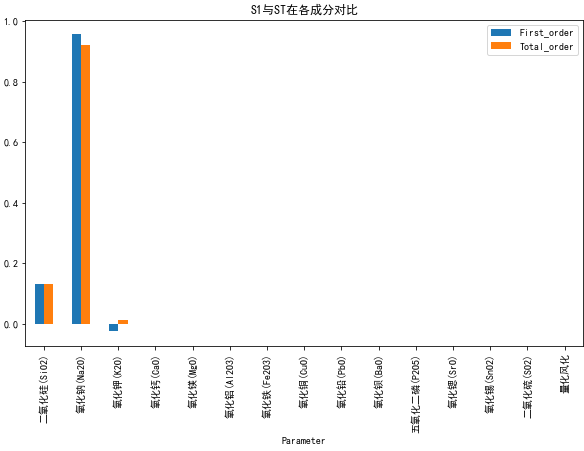
\includegraphics[width=1\textwidth,height=0.7\textwidth]{img/S1_2.png} % 图片相对位置 
	\caption{第三问一阶灵敏性分析} % 图片标题 
	\label{fig:figure 9} % 图片标签
\end{figure}

计算$SiO_2,Na_2O,K_2O$之间的交互作用:

\[\left\{\begin{array}{llcl}
    SiO_2-Na_2O = -0.021632681100776097      \\
SiO_2-K_2O =	0.030570028332032845		\\
Na_2O-K_2O =-0.04295463009829131
\end{array} \right.\]


% \left\{
% \begin{array}{rcl}
% SiO_2-Na_2O = -0.021632681100776097      \\
% SiO_2-K_2O =	0.030570028332032845		\\
% Na_2O-K_2O =-0.04295463009829131
% \end{array} \right.

$SiO_2-Na_2O$以及$Na_2O-K_2O$的指数都小于0,说明随着样本数量的增加,它们的误差会不断减小。$SiO_2-K_2O$的指标为正,说明两者之间具有较强的关联性,会出现计算误差。
二阶灵敏度表示处理两个参数组合下的灵敏度变换,故此通过热力图进行可视化分析,我们可以发现二阶交互作用很小,所有指数的值都小于0.04,成分$K_2O$的二阶灵敏度最高。

\begin{figure}[H]\centering
	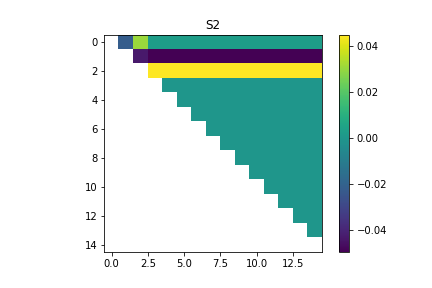
\includegraphics[width=1\textwidth,height=0.6\textwidth]{img/S2_heatmap2.png} % 图片相对位置 
	\caption{第三问二阶灵敏性分析} % 图片标题 
	\label{fig:figure 9} % 图片标签
\end{figure}






%第八部分
\section{问题四的模型建立与求解}
\subsection{问题分析}
第四问可以细分为两个小问,即分别是:1.按照不同的的类别划分玻璃文物样品,并对已划分的样品之间的
化学成分进行关联性分析;2.分析已划分类别样品中的化学成分的关联关系的差异性。

第一,按照类型划分出高钾玻璃文物和铅钡玻璃文物两种样品群,缺失值处理与问题一相同。采用随机森林
进行填补,过程不再赘述。对所有的定量数据进行归一化处理后进行灰色关联分析,分析出成分之间的关联
关系。

第二,因为样本分类为不同类别后单个样本群数据较少,所以选择使用非参数检验的方法进行关联关系的差异性
研究。对原始数据进行随机森林填补和归一化处理后,判断是否服从正太分布后进行多配对样本Friedman检验
,分析出成分之间的关联关系的差异性。

\subsection{灰色关联分析模型的建立}
\subsubsection{模型确立}
在现实的客观世界中,存在着多种相互影响的因素。但是由于客观世界的制约,许多因素的关系无法直接
可见,即是属于灰色的,无法清晰地辨别这些因素可能存在的各种密切关系,会对未来对这些因素的分析造成
各种困难,不易找到主要的矛盾和特性。而灰色关联分析的目的就是定量的表述出各种因素之间存在的关联程度
,以便揭示出这些因素组成的灰色系统的主要矛盾和特性。

\subsubsection{数据线性判断}
判断出数据是否线性是选择模型的前提条件。通过对数据的线性诊断可以判断出数据是否符合所选的模型要求
。根据问题一的共线性诊断结论,各成分之间存在严重的共线性问题,即各个变量可能表示为一个变量,
无需分析线性相关,无法通过线性回归确定各个变量的紧密程度。因为灰色关联分析适用于对一个系统发
展变化态势的定量描述和比较的方法,更加客观地定量表达事物之间的关联程度,故选择此模型。

\subsubsection{模型构建}
第一步需要确定分析数列。首先确定反映系统行为特征的参考数列和影响系统行为的比较数列。
通常称第一种序列为参考数列。后一种数列称比较数列。

参考序列(母序列)公式为:
\begin{equation}
	W=W(k) \mid k=1,2\dots n
\end{equation}

比较序列(子序列)公式为:
\begin{equation}
	S_{i}=S_{i}(k) \mid k=1,2 \ldots n,i=1,2 \ldots m
\end{equation}

第二步,对变量进行无量纲化处理。由于系统中的各种因素的数据量纲可能不同,会造成比较结果较差甚至
无法正确得到结果的情况。因此在进行灰色关联分析的适合,首先要进行数据的无量纲化处理。本文采用的是
均值化处理的方法。

均值化处理公式:
\begin{equation}
	D_{i}(k)=\frac{D_{i}(k)}{D_{i}}, k=1,2 \ldots n;i=1,2 \ldots m
\end{equation}

其中k对应时间段, i对应比较数列中的第i行。

第三步,计算关联系数。公式如下:
\begin{equation}
	\xi_{i}(k)=\frac{\min _{i} \min _{k}\left|a(k)-b_{i}(k)\right|+\rho \max _{i} \max _{k}\left|a(k)-b_{i}(k)\right|}{\left|a(k)-b_{i}(k)\right|+\rho \max _{i} \max _{k}\left|a(k)-b_{i}(k)\right|}
\end{equation}

其中$\rho \in(0, \infty)$,$\rho$称为分辨系数。而$\rho$的大小决定分辨能力,分辨能力随$\rho$的增大
而增大,反之亦然。一般$\rho$的取值是(0,1)。当$\rho\mathbf{\le }0.5463$时,分辨能力最好。本文取0.5.

第四步,计算关联度。关联系数时母序列和子序列在各个时刻的关联程度值,所以这个值不只有一个。但是由于
值过多会导致信息分散,不便于进行整体的比较,因此对各个时刻的关联系数集中为一个平均值是十分必要的
。作为母序列和子序列的关联程度的该值的公式如下:
\begin{equation}
    r_{i}=\frac{1}{n} \sum_{k=1}^{n} \xi_{i}(k), k=1,2 \ldots n
\end{equation}

第五步,关联度排序。在构建模型的最后需要对关联度按大小排序,当$r_{i}$在算出$W(k)$与$S_{i}(k)$
两个母子序列的关联系数后,计算各类关联系数的平均值,即为关联度。

\subsection{灰色关联模型的求解}
\subsubsection{模型求解分析}
在对数据进行共线性诊断后得到数据是不服从线性的信息后,即得选择灰色关联分析
的合理性。该模型可以预测线性关系非常弱,无法通过线性分析完成
紧密程度分析的变量关系。灰色关联度分析更加注重事物发展过程的相似性与相近性
,能更加客观地定量表达变量之间的关联程度,解决了本体的成分之间的问题。

本问运用了灰色关联分析模型解决的问题是针对不同类别的玻璃文物样品,分析其
化学成分之间的关联关系。通过确定以及遍历所有的成分成为母序列后,与没有成为
母序列的所有其他成分组成的子序列构成每一次的灰色关联分析模型。由于共有
14项成分,最后得到共14份不同的关联关系表。在此节选二氧化硅的求解过程
,其余成分的关联关系结果详见附录。

约定二氧化硅、氧化钠、氧化钾、氧化钙、氧化镁、氧化铝、氧化铁、氧化铜、氧化铁、
氧化铅、氧化钡、五氧化二磷、氧化锶、氧化锡、二氧化硫、表面风化这些数据指标
以$x_1$,$x_2$,$x_3$ \dots $x_{16}$表示。

\subsubsection{求解过程}
\textbf{Step1:数据预处理}

在进行灰色关联分析前需要进行去量纲化处理。共有两种处理方法可以选择:1.初值化
:稳定递增或者递减的数据;2.均值化:没有明显升降趋势的数据。根据附件提供的数据进行描述性
统计,观察所有成分的散点图图像,得出结论:数据没有稳定增长或者减少,故选择均值化
操作。下图为二氧化硅散点图,其余样本描述性统计图像详见附录。
\begin{figure}[H]\centering
	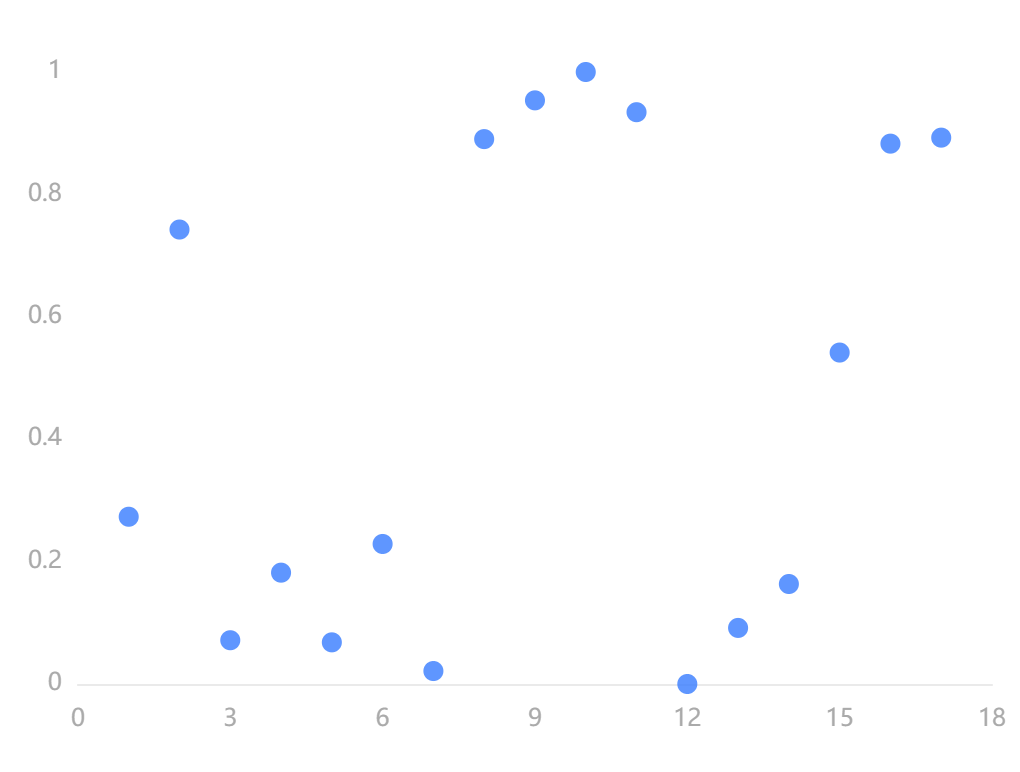
\includegraphics[width=0.5\textwidth]{img/二氧化硅标准化散点图.png} % 图片相对位置 
	\caption{二氧化硅标准化散点图} % 图片标题 
	\label{fig:figure 3} % 图片标签
\end{figure}

\textbf{Step2:类别划分}

本题要求按照不同的类别进行关联关系的分析。类别的划分参照类型和表面风化两个属性进行
确定。其中,类型为第一级,表面是否风化是第二级。最后划分出四个类别进行分析。

\textbf{Step3:灰色关联系数}

以二氧化硅为母序列,针对13个评价项以及17项数据进行灰色关联度分析,研究母序列与13个子序列
的关联关系。并基于关联度提供分析参考,使用灰色关联度分析时,分辨系数取0.5,
结合关联系数计算公式计算出关联系数值,并根据关联系数值,然后计算出如下关联度值,并用于评价判断。
关联系数的小数位数设置为2,以方便展示,具体数值详见附录。
\begin{table}[!ht]
    \centering
    \caption{高钾玻璃-二氧化硅灰色关联系数}
    \begin{tabular}{|l|l|l|l|l|l|l|l|l|l|l|l|l|l|}
    \hline
        索引项 & x1 & x2 & x3 & x4 & x5 & x6 & x7 & x8 & x9 & x10 & x11 & x12 & x13 \\ \hline
        无风化 & 0.71  & 0.78  & 0.76  & 0.98  & 0.95  & 0.84  & 0.67  & 0.94  & 0.77  & 0.86  & 0.91  & 0.88  & 0.84  \\ \hline
        无风化 & 0.71  & 0.77  & 0.72  & 0.79  & 0.79  & 0.73  & 0.68  & 0.66  & 0.75  & 0.74  & 0.82  & 0.74  & 0.71  \\ \hline
        无风化 & 0.64  & 0.64  & 0.70  & 0.76  & 0.76  & 0.69  & 0.53  & 0.94  & 0.85  & 0.87  & 0.85  & 0.97  & 0.99  \\ \hline
        无风化 & 0.73  & 0.75  & 0.69  & 0.65  & 0.76  & 0.75  & 0.83  & 0.92  & 0.96  & 0.91  & 0.96  & 0.66  & 0.89  \\ \hline
        无风化 & 0.67  & 0.67  & 0.65  & 0.57  & 0.67  & 0.64  & 0.66  & 0.98  & 0.88  & 0.81  & 0.97  & 0.64  & 0.98  \\ \hline
        无风化 & 0.76  & 0.84  & 0.76  & 0.57  & 0.60  & 0.72  & 0.80  & 0.87  & 0.95  & 0.44  & 0.90  & 0.78  & 0.90  \\ \hline
        无风化 & 0.69  & 0.74  & 0.71  & 0.57  & 0.58  & 0.41  & 0.75  & 1.00  & 0.94  & 0.39  & 0.77  & 0.66  & 0.95  \\ \hline
        风化 & 0.94  & 0.64  & 0.64  & 0.65  & 0.65  & 0.61  & 0.92  & 1.00  & 0.83  & 0.68  & 0.79  & 0.65  & 1.00  \\ \hline
        风化 & 0.66  & 0.59  & 0.61  & 0.63  & 0.61  & 0.61  & 0.68  & 0.93  & 0.95  & 0.62  & 0.80  & 0.62  & 0.98  \\ \hline
        风化 & 0.68  & 0.59  & 0.58  & 0.63  & 0.58  & 0.59  & 0.61  & 0.90  & 0.91  & 0.61  & 0.97  & 0.60  & 0.83  \\ \hline
        风化 & 0.66  & 0.61  & 0.61  & 0.64  & 0.62  & 0.61  & 0.70  & 1.00  & 0.78  & 0.60  & 0.83  & 0.63  & 0.99  \\ \hline
        无风化 & 0.80  & 0.62  & 0.59  & 0.69  & 0.70  & 0.60  & 0.54  & 0.87  & 0.57  & 0.71  & 0.56  & 0.89  & 0.86  \\ \hline
        无风化 & 0.73  & 0.65  & 0.62  & 0.98  & 0.62  & 0.99  & 0.94  & 0.93  & 0.91  & 0.94  & 0.79  & 0.94  & 0.73  \\ \hline
        无风化 & 0.90  & 0.62  & 0.64  & 0.90  & 0.76  & 0.95  & 1.00  & 0.90  & 0.90  & 0.94  & 0.90  & 0.95  & 0.77  \\ \hline
        无风化 & 0.78  & 0.94  & 0.78  & 0.80  & 0.83  & 0.82  & 0.77  & 0.69  & 0.99  & 0.96  & 0.79  & 0.33  & 0.80  \\ \hline
        风化 & 0.73  & 0.61  & 0.66  & 0.64  & 0.71  & 0.63  & 0.62  & 0.83  & 0.82  & 0.62  & 0.84  & 0.64  & 0.98  \\ \hline
        风化 & 0.67  & 0.65  & 0.63  & 0.61  & 0.66  & 0.61  & 0.70  & 0.96  & 0.78  & 0.64  & 0.76  & 0.64  & 0.99  \\ \hline
    \end{tabular}
\end{table}

同样的操作过后得到铅钡玻璃-二氧化硅的灰色关联系数表。因为数据过多,故截取部分数据展示,其余
数据详见附录如下所示:
\begin{table}[!ht]
    \centering
    \caption{铅钡玻璃-二氧化硅灰色关联系数}
    \begin{tabular}{|l|l|l|l|l|l|l|l|l|l|l|l|l|l|}
    \hline
        索引项 & x1 & x2 & x3 & x4 & x5 & x6 & x7 & x8 & x9 & x10 & x11 & x12 & x13 \\ \hline
        风化 & 0.94  & 0.67  & 0.98  & 0.88  & 0.79  & 0.74  & 0.76  & 0.80  & 0.91  & 1.00  & 0.80  & 0.96  & 0.86  \\ \hline
        风化 & 0.68  & 0.99  & 0.97  & 0.95  & 0.93  & 0.97  & 0.37  & 0.89  & 0.49  & 0.85  & 0.87  & 0.86  & 0.91  \\ \hline
        风化 & 0.61  & 0.82  & 0.66  & 0.82  & 0.94  & 0.84  & 0.64  & 0.74  & 0.46  & 0.57  & 0.66  & 0.75  & 0.41  \\ \hline
        风化 & 0.76  & 0.81  & 0.79  & 0.87  & 0.95  & 0.98  & 0.63  & 0.94  & 0.83  & 0.62  & 1.00  & 0.98  & 0.98  \\ \hline
        风化 & 0.89  & 0.99  & 0.83  & 0.84  & 0.92  & 0.83  & 0.74  & 0.80  & 0.88  & 0.62  & 0.84  & 0.93  & 0.86  \\ \hline
        无风化 & 0.84  & 0.85  & 0.64  & 0.94  & 0.82  & 0.84  & 0.66  & 0.74  & 0.65  & 0.83  & 0.86  & 0.90  & 0.84  \\ \hline
        无风化 & 0.69  & 0.69  & 0.66  & 0.73  & 0.70  & 0.72  & 1.00  & 0.71  & 0.89  & 0.67  & 0.79  & 0.83  & 0.95  \\ \hline
        无风化 & 0.70  & 0.82  & 0.78  & 0.94  & 0.86  & 0.91  & 0.44  & 0.99  & 0.58  & 0.77  & 0.59  & 0.97  & 0.75  \\ \hline
        无风化 & 0.78  & 0.79  & 0.69  & 0.78  & 0.75  & 0.94  & 0.76  & 0.87  & 0.77  & 0.67  & 0.72  & 0.83  & 0.79  \\ \hline
    \end{tabular}
\end{table}

\textbf{Step4:灰色关联度}

关联度表示各评价项与母序列之间的相似关联程度,其是由关联系数进行计算平均值得出,
关联度值介于0~1之间,该值越大表示评价项与母序列相关性越强,关联度越高,意味着评价项
与母序列之间关系越紧密,因而其评价越高。结合关联度值,针对所有评价项进行排序,得到各评价项排名。
最后的结果展示如下表

\begin{minipage}{\textwidth}
    \begin{minipage}[t]{0.48\textwidth}
    \makeatletter\def\@captype{table}
    \caption{高钾玻璃-二氧化硅灰色关联度}
    ~~~~~~~~~~~~~~~~\begin{tabular}{|c|c|c|}
        \hline
         评价项 & 关联度 & 排名 \\ \hline
            $x_{2}$ & 0.812 & 4 \\ \hline
            $x_{3}$ & 0.758 & 9 \\ \hline
            $x_{4}$ & 0.748 & 12 \\ \hline
            $x_{5}$ & 0.832 & 3 \\ \hline
            $x_{6}$ & 0.834 & 2 \\ \hline
            $x_{7}$ & 0.807 & 5 \\ \hline
            $x_{8}$ & 0.757 & 10 \\ \hline
            $x_{9}$ & 0.754 & 11 \\ \hline
            $x_{10}$ & 0.793 & 6 \\ \hline
            $x_{11}$ & 0.708 & 13 \\ \hline
            $x_{12}$ & 0.759 & 8 \\ \hline
            $x_{13}$ & 0.856 & 1 \\ \hline
            $x_{14}$ & 0.761 & 7 \\ \hline
    \end{tabular}
    \label{sample-table}
    \end{minipage}
    \begin{minipage}[t]{0.48\textwidth}
    \makeatletter\def\@captype{table}
    \caption{铅钡玻璃-二氧化硅灰色关联度}
    ~~~~~~~~~~~~~~~~\begin{tabular}{|c|c|c|}
        \hline
            评价项 & 关联度 & 排名 \\ \hline
            $x_{2}$ & 0.812 & 4 \\ \hline
            $x_{3}$ & 0.758 & 9 \\ \hline
            $x_{4}$ & 0.748 & 12 \\ \hline
            $x_{5}$ & 0.832 & 3 \\ \hline
            $x_{6}$ & 0.834 & 2 \\ \hline
            $x_{7}$ & 0.807 & 5 \\ \hline
            $x_{8}$ & 0.757 & 10 \\ \hline
            $x_{9}$ & 0.754 & 11 \\ \hline
            $x_{10}$ & 0.793 & 6 \\ \hline
            $x_{11}$ & 0.708 & 13 \\ \hline
            $x_{12}$ & 0.759 & 8 \\ \hline
            $x_{13}$ & 0.856 & 1 \\ \hline
            $x_{14}$ & 0.761 & 7 \\ \hline
    \end{tabular}
    \end{minipage}
    \end{minipage}
~\\

总和两表可以发现,铅钡玻璃的其余成分与二氧化硅关联密切的有氧化锡、氧化铝、氧化镁、氧化纳、
氧化铁等,而高钾玻璃的其余成分与二氧化硅关系密切的有氧化铅、二氧化硫、氧化钡、氧化锶等物质。
不同的类别玻璃的成分之间的关联性差别巨大,是否风化也影响着同一种玻璃的成分关联关系。例如:高钾玻璃
中风化玻璃中二氧化硅与二氧化硫、氧化铜的关联关系更加紧密;而未风化的玻璃则与氧化钙、氧化铜
、氧化钡、氧化锶、二氧化硫的关系更为紧密。详细的比较关联数据详见附录。


\subsection{多配对样本Friedman检验-Nemenyi后续检验}
\subsubsection{模型确立}
对于已分类别的四类样本数据,因为样本数据的成分之间存在着某种关系
,因此对于差异化的检验需要进行非参数检验中非独立的检验方法的同时
还需要该模型能够分析样本群中各个样本之间的关系。多配对样本Friedman检验
是一种非参数检验的方法,该种方法使用秩次和秩对样本排序后并进行统计
各个样本之间显著性差异的一种方法。

多配对样本Friedman检验单一使用略显单薄,为了使数据更加明确,我们引进Nemenyi 后续检验。
Nemenyi是一种用于
多样本进行两两比较的一种算法,能够弥补只使用Friedman模型的
局限性。混合两种模型后样本的差异性
分析能够解决测试的样本群上和各个成分之间的差异性分析问题。

\subsubsection{求解过程}
\textbf{Step1:多配对样本Friedman检验}

将各个成分的占比转换成成分对应的秩次并统计秩和,接着样本群的所有成分
进行显著性差异分析,计算出统计量。但是可能会出现秩的值是一样的情况
,对此我们进行校正,校正公式如下:
\begin{equation}
    F^{\prime}=\frac{F}{1-H /\left[JS\left(S^{2}-1\right)\right]}
\end{equation}

在公式中,$F^{\prime}$是校正量;$H=\sum_{i=1}^{n}(n_{i}^{3}-n_{i})$
中的$n_{i}$是每一个秩组出现的相同秩值的成分数,如果未出现则i=1。

Friedman检验是根据J、S、a(显著性水平)的值与Friedman临界值表中的
$F_{0}$,若统计量F或者修正量大于或等于$F_{0}$,则该成分在整体
上有显著性差异。

将处理后的数据带入模型中,得到如下的结果:
\begin{table}[!ht]
    \centering
    \begin{tabular}{|l|l|l|l|l|l|l|}
    \hline
        变量名 & 样本量 & 中位数 & 标准差 & 统计量 & p值(双尾) & Cohen's f值 \\ \hline
        $x_{1}$ & 49 & 0.447 & 0.26 &  \multirow{14}{*}{109.319} &  \multirow{14}{*}{0.000***} &  \multirow{14}{*}{0.386} \\ \cline{1-4}
        $x_{2}$ & 49 & 0.315 & 0.207 & ~ & ~ & ~ \\ \cline{1-4}
        $x_{3}$ & 49 & 0.082 & 0.247 & ~ & ~ & ~ \\ \cline{1-4}
        $x_{4}$ & 49 & 0.284 & 0.269 & ~ & ~ & ~ \\ \cline{1-4}
        $x_{5}$ & 49 & 0.186 & 0.183 & ~ & ~ & ~ \\ \cline{1-4}
        $x_{6}$ & 49 & 0.188 & 0.217 & ~ & ~ & ~ \\ \cline{1-4}
        $x_{7}$ & 49 & 0.156 & 0.181 & ~ & ~ & ~ \\ \cline{1-4}
        $x_{8}$ & 49 & 0.097 & 0.234 & ~ & ~ & ~ \\ \cline{1-4}
        $x_{9}$ & 49 & 0.371 & 0.245 & ~ & ~ & ~ \\ \cline{1-4}
        $x_{10}$ & 49 & 0.207 & 0.237 & ~ & ~ & ~ \\ \cline{1-4}
        $x_{11}$ & 49 & 0.176 & 0.274 & ~ & ~ & ~ \\ \cline{1-4}
        $x_{12}$ & 49 & 0.235 & 0.21 & ~ & ~ & ~ \\ \cline{1-4}
        $x_{13}$ & 49 & 0.304 & 0.156 & ~ & ~ & ~ \\ \cline{1-4}
        $x_{14}$ & 49 & 0.239 & 0.204 & ~ & ~ & ~ \\ \cline{1-4}
        \hline
    \end{tabular}
\end{table}

上表展示了Friedman检验的结果,包括中位数、统计量与效应量Cohen's f值。
分析过程如下:

1.分析每个分析项是否小于0.05或者0.01;

2.若呈显著性,拒绝原假设,说明两组数据之间存在显著性差异,可以根据中位数±标准差的方式对差异进行分析,反之则表明数据不呈现差异性;

3.Cohen's f值: 表示效应量大小,效应量小、中、大的区分临界点分别是:0.1、0.25和0.40。

通过Friedman检验分析结果表可知,显著性p值为0.000***<0.05,因此统计结果显著,
说明二氧化硅、氧化钠、氧化钾等14个成分之间存在显著差异;
其差异幅度Cohen's f值为:0.386,差异幅度较小。

\textbf{Step2:Nemenyi后续检验}

Nemenyi后续检验的流程是两两比较后得到与Friedman检验属性相同的其他值结果。将样本
带入模型中后得到事后比较表。由于数据较多,本问中只演示二氧化硅与其他成分的两两比较
结果,其余结果详见附录。二氧化硅事后比较表如下:

\begin{table}[H]
    \centering
	\caption{二氧化硅事后比较表}
    \begin{tabular}{|c|c|c|c|c|c|c|}
    \hline
	\multirow{2}{*}{配对变量} & \multicolumn{3}{|c|}{中位数±标准差} & \multirow{2}{*}{统计量} & \multirow{2}{*}{P值} & \multirow{2}{*}{Cohen's d}\\ \cline{2-4}
        ~ & 配对1 & 配对2 & 配对差值(配对1-配对2) & ~ & ~ & ~  \\ \hline
        $x_{2}$ & 0.447±0.26 & 0.315±0.207 & 0.132±0.053 & 0.956 & 0.9 & 0.47 \\ \hline
        $x_{3}$ & 0.447±0.26 & 0.082±0.247 & 0.364±0.013 & 9.664 & 0.001*** & 1.281 \\ \hline
        $x_{4}$ & 0.447±0.26 & 0.284±0.269 & 0.163±0.009 & 3.159 & 0.589 & 0.601 \\ \hline
        $x_{5}$ & 0.447±0.26 & 0.186±0.183 & 0.261±0.076 & 5.02 & 0.026** & 1.109 \\ \hline
        $x_{6}$ & 0.447±0.26 & 0.188±0.217 & 0.259±0.043 & 5.942 & 0.002*** & 1.079 \\ \hline
        $x_{7}$ & 0.447±0.26 & 0.156±0.181 & 0.29±0.078 & 6.488 & 0.001*** & 1.265 \\ \hline
        $x_{8}$ & 0.447±0.26 & 0.097±0.234 & 0.35±0.026 & 8.332 & 0.001*** & 1.202 \\ \hline
        $x_{9}$ & 0.447±0.26 & 0.371±0.245 & 0.076±0.014 & 0.581 & 0.9 & 0.375 \\ \hline
        $x_{10}$ & 0.447±0.26 & 0.207±0.237 & 0.24±0.023 & 4.747 & 0.050** & 0.892 \\ \hline
        $x_{11}$ & 0.447±0.26 & 0.176±0.274 & 0.271±0.014 & 6.01 & 0.002*** & 0.842 \\ \hline
        $x_{12}$ & 0.447±0.26 & 0.235±0.21 & 0.212±0.049 & 3.586 & 0.386 & 0.829 \\ \hline
        $x_{13}$ & 0.447±0.26 & 0.304±0.156 & 0.142±0.104 & 1.964 & 0.9 & 0.717 \\ \hline
        $x_{14}$ & 0.447±0.26 & 0.239±0.204 & 0.207±0.055 & 5.942 & 0.002*** & 1.077 \\ \hline
    \end{tabular}
\end{table}
得出例如如下的结论:
二氧化硅对于氧化钠,显著性P值为0.900,水平上呈现不显著性,不能拒绝原假设,因此二氧化硅和氧化钠之间不存在显著性差异。

总结为:氧化纳、氧化钙、氧化铅、氧化锶、氧化锡对二氧化硅不存在显著性差异;其余的成分都与二氧化硅有显著性差异。
%此处看情况,多少个模型写多少个评价
\section{模型的评价}
\subsection{模型一}
\noindent \textbf{优点:}

1.定性定量分析数据,结合离散型数据的特点进行显著性和相关性检验,得出有效的结论。

2.采用随机森林进行了数据的预测和填补利用机器学习来弥补人工给出的数据中存在的误差,对填补后仍有一定偏差的数据又进行了降低误差的处理,
通过对误差函数的加权处理使其数据更加真实;同时归一化去除量纲,给出了一定的误差填补范围,使得数据更加可靠。

3.通过诊断发现数据具有很强的多重共线性问题,岭回归分析预测模型是优化过的最小二乘估计,属于有偏估计,
适用于解决多重共线性的回归方法,得出的结果拟合效果极佳。


\noindent \textbf{缺点:}

1.数据指标之间存在较强的共线性关系,没有能够充分挖掘其价值。

2.岭回归分析预测模型给出的化学指标之间的统计规律需拟合的方程数目过多。

3.算法也会存在误差,填补过程给出的误差范围有一定的主观性。

\subsection{模型二}

\noindent \textbf{优点:}

1.混合$K-means++$和$BP$神经网络使用,$BP$神经网络很好的改善了$K-means++$在分类过程中出现的一些偏离较大的值(分类不理想)。

2.遗传算法的寻优效果较好,能够精准的找到全局最优解,据此进行的调参使得神经网络模型整体更加完善,分析预测效果精准。

3.随机采样处理利于降低模型的整体误差性。


\noindent \textbf{缺点:}

1.$K-means++$单独聚类高钾的结果不够理想,有部分偏离的值。

2.遗传算法的时间复杂度不小,在数据集过多时,会由于时间过长搜寻不到最优解。


\subsection{模型三}
\textbf{优点:}

1.集成多个成员模型,采用随机森林算法来对决策树进行抉择,得出的结果总是比决策树更优,属于全局最优。

2.集成学习过程中重采样能够很好的解决许多不同应用中的不均衡数据集问题。经过穷举寻优找到准确且多样化的成员时,较利于最终集成性能和泛化能力的提高。

3.投票加权平均的机制能够有效的降低多个模型的方差,模型的鲁棒性较高。

4.最终$VoteModel$模型的多种准确率都为1,泛化能力强,敏感性低,十分完美的契合。

\textbf{缺点:}

1.集成模型中所涉及的模型过多,涉及的数据集较少的情况下,单个模型之间的稳定性差,容易受到干扰和噪声,较为敏感。

2.$Exhaustive search$时间复杂度大,当数据量过大时,会存在难以找到最优的情况。

\subsection{模型四}
\textbf{优点:}


\textbf{缺点:}


%第十部分
\section{参考文献}
% \noindent{[1]姜启源,谢金星,叶俊,数学模型(第四版),北京:高等教育出版社,2011.1}

% \noindent{[2] 司宛玲,司守奎,数学建模简明教程[M]北京:国防工业出版社,2019,185-189}

% \noindent{[3] 韩中庚,数学建模方法及其应用(第二版)[M]北京:高等教育出版社,2010,163-171}

\begin{thebibliography}{100}

    \bibitem{ref1}李青会,黄教珍,李飞,干福熹.中国出土的一批战国古玻璃样品化学成分的检测[J].文物保护与考古科学,2006(02):8-13.DOI:10.16334/j.cnki.cn31-1652/k.2006.02.002.
    \bibitem{ref2}于群,霍筱东,何剑,李琳,张建新,冯煜尧.基于斯皮尔曼相关系数和系统惯量的中国电网停电事故趋势预测[JOL].中国电机工程学报1-12[2022-09-16].httpkns.cnki.netkcmsdetail11.2107.TM.20220824.1625.012.html
    \bibitem{ref3}:ictor Henrique Alves Ribeiro and Gilberto Reynoso-Meza. 2020. Ensemble learning by means of a multi-objective optimization design approach for dealing with imbalanced data sets.Exp. Syst. Applic.147 (2020), 113232.
    \bibitem{ref4}Shenkai Gu and Yaochu Jin. 2014. Generating diverse and accurate classifier ensembles using multi-objective op-timization. InProceedings of the IEEE Symposium on Computational Intelligence in Multi-Criteria Decision-Making(MCDM). IEEE, 9–15.
    \bibitem{ref5}
    
    \end{thebibliography}
\noindent{}
\noindent{}













\newpage %参考文献完后重启一页




% \clearpage
% \bibliographystyle{plain}
% \bibliography{ref}%ref指向自己创建的ref.bib
% % IoU\cite{zheng2020distance}
% \clearpage

%最后一部分
\section{附录}
\subsection{代码}

\lstset{language=python}
\begin{lstlisting}
	
\end{lstlisting}


\end{document}
